\chapter{Evoluindo uma plataforma de rede social}
\label{evol-rede-social}

Neste capítulo é discutida a plataforma Noosfero, desde sua arquitetura até os processos de desenvolvimento da comunidade. Além disso, é apresentado o Comunidade.UnB, rede de colaboração livre, no qual são propostas evoluções para que se torne um ambiente híbrido utilizado por professores e alunos.

\section{Noosfero}
\label{noosfero}

O Noosfero \footnote{Disponível em: \url{http://www.noosfero.org}} é uma plataforma livre para criação de redes sociais, desenvolvida em 2007, pela Cooperativa de Tecnologias Livres - Colivre \footnote{Disponível em: \url{http://www.colivre.coop.br}}, sob a licença AGPL\footnote{Licença de software GNU} V3, com a proposta de facilitar a criação de redes sociais personalizadas, livres e autônomas e a geração de conteúdo colaborativo.

Além das funcionalidades de rede social, com foco na produção e compartilhamento de conteúdo, o Noosfero permite que dentro da rede cada usuário e comunidade tenha o seu espaço com total flexibilidade de personalização visual e gerenciamento de conteúdo. São exemplos de portais que utilizam o Noosfero: o Participa BR \footnote{Disponível em: \url{https://www.participa.br/}}, Stoa\footnote{Disponível em: \url{http://stoa.usp.br/}}, Portal da FGA\footnote{Disponível em: \url{http://fga.unb.br/}} e o novo Portal do Software público Brasileiro \footnote{Disponível em: \url{https://portal.softwarepublico.gov.br/}}.

O Noosfero foi desenvolvido na linguagem de programação Ruby, atualmente na versão 2.2.0, e utiliza o \textit{framework} aplicações web \textit{Ruby on Rails} \footnote{Disponível em: \url{http://rubyonrails.org/}}, versão 3.2.21. E utiliza também padrões arquiteturais de software Model-View-Controller (MVC), e o padrão de plugins que serão apresentados na seção \ref{arquitetura}.

A escolha da linguagem \textit{Ruby} foi decisiva no Noosfero, pois possui uma sintaxe simples, que facilita a manutenibilidade do sistema, característica importante em projetos de software livre que tendem a atrair colaboradores externos \cite{meirelles2013}. A escolha do \textit{Rails} foi influenciada pelos seus conceitos básicos que auxiliam em sua produtividade: ``Não Repita a Si Mesmo'' (DRY-\textit{Don't Repeat Yourself}) e ``convenção sobre configuração'' (\textit{Convention Over Configuration}) \cite{akita2006repensando}. Além disso , por questões de segurança, o Noosfero é homologado para a versão \textit{stable} do \textit{Debian}, acompanhando a versão do \textit{Ruby} e do \textit{Rails} dessa distro.

\subsection{Práticas de desenvolvimento da comunidade Noosfero}
\label{proc-desenvol-comunidade}
% - ciclos
% - repositorio
% - commiters/revisao
% - testes

Para que novos desenvolvedores colaborem com o Noosfero, a comunidade utiliza em seu próprio \textit{site} uma seção para o desenvolvimento. Nessa seção, encontram-se os manuais com os passos para instalação do ambiente, descrição dos \textit{plugins} disponíveis, instruções para a personalização da plataforma através de temas além de informações arquiteturais da plataforma. Para realizar o controle de itens a fazer, como a implementação de novas funcionalidades ou correção de bugs é utilizado um \textit{Issue Tracker} do repositório oficial no GitLab \footnote{Disponível em: \url{https://gitlab.com/noosfero/noosfero}}.

Uma vez que o desenvolvedor ou usuário tenha registro no GitLab, é possível utilizar o \textit{Issue Tracker} para cadastrar novas funcionalidades ou \textit{bugs} de maneira simples seguindo os seguintes passos:

\begin{enumerate}
\item preencher o campo título;
\item definir a descrição do item, se existir, é necessário especificar com qual \textit{plugin} o item está relacionado;
\item associar um desenvolvedor responsável pela sua implementação \textit{issue};
\item definir as \textit{labels} da funcionalidade, onde é especificado ao que está relacionado a nova \textit{issue}.
\end{enumerate}

Após a criação da \textit{issue}, todos os membros da comunidade podem visualizar os dados e especificações, bem como discutir sobre os propósitos e formas de implementação da funcionalidade.

A Figura \ref{issue-tracker} evidencia o \textit{Issue Tracker} do Noosfero onde é possível verificar os itens que foram mapeados e seus respectivos \textit{status}, se ainda estão abertas ou fechadas, além de um filtro para os autores e os marcadores envolvidos à cada uma delas. Dessa forma, é possível priorizar os itens identificados como sendo de maior importância para os usuários e desenvolvedores.

\begin{figure}[h]
    \centering
    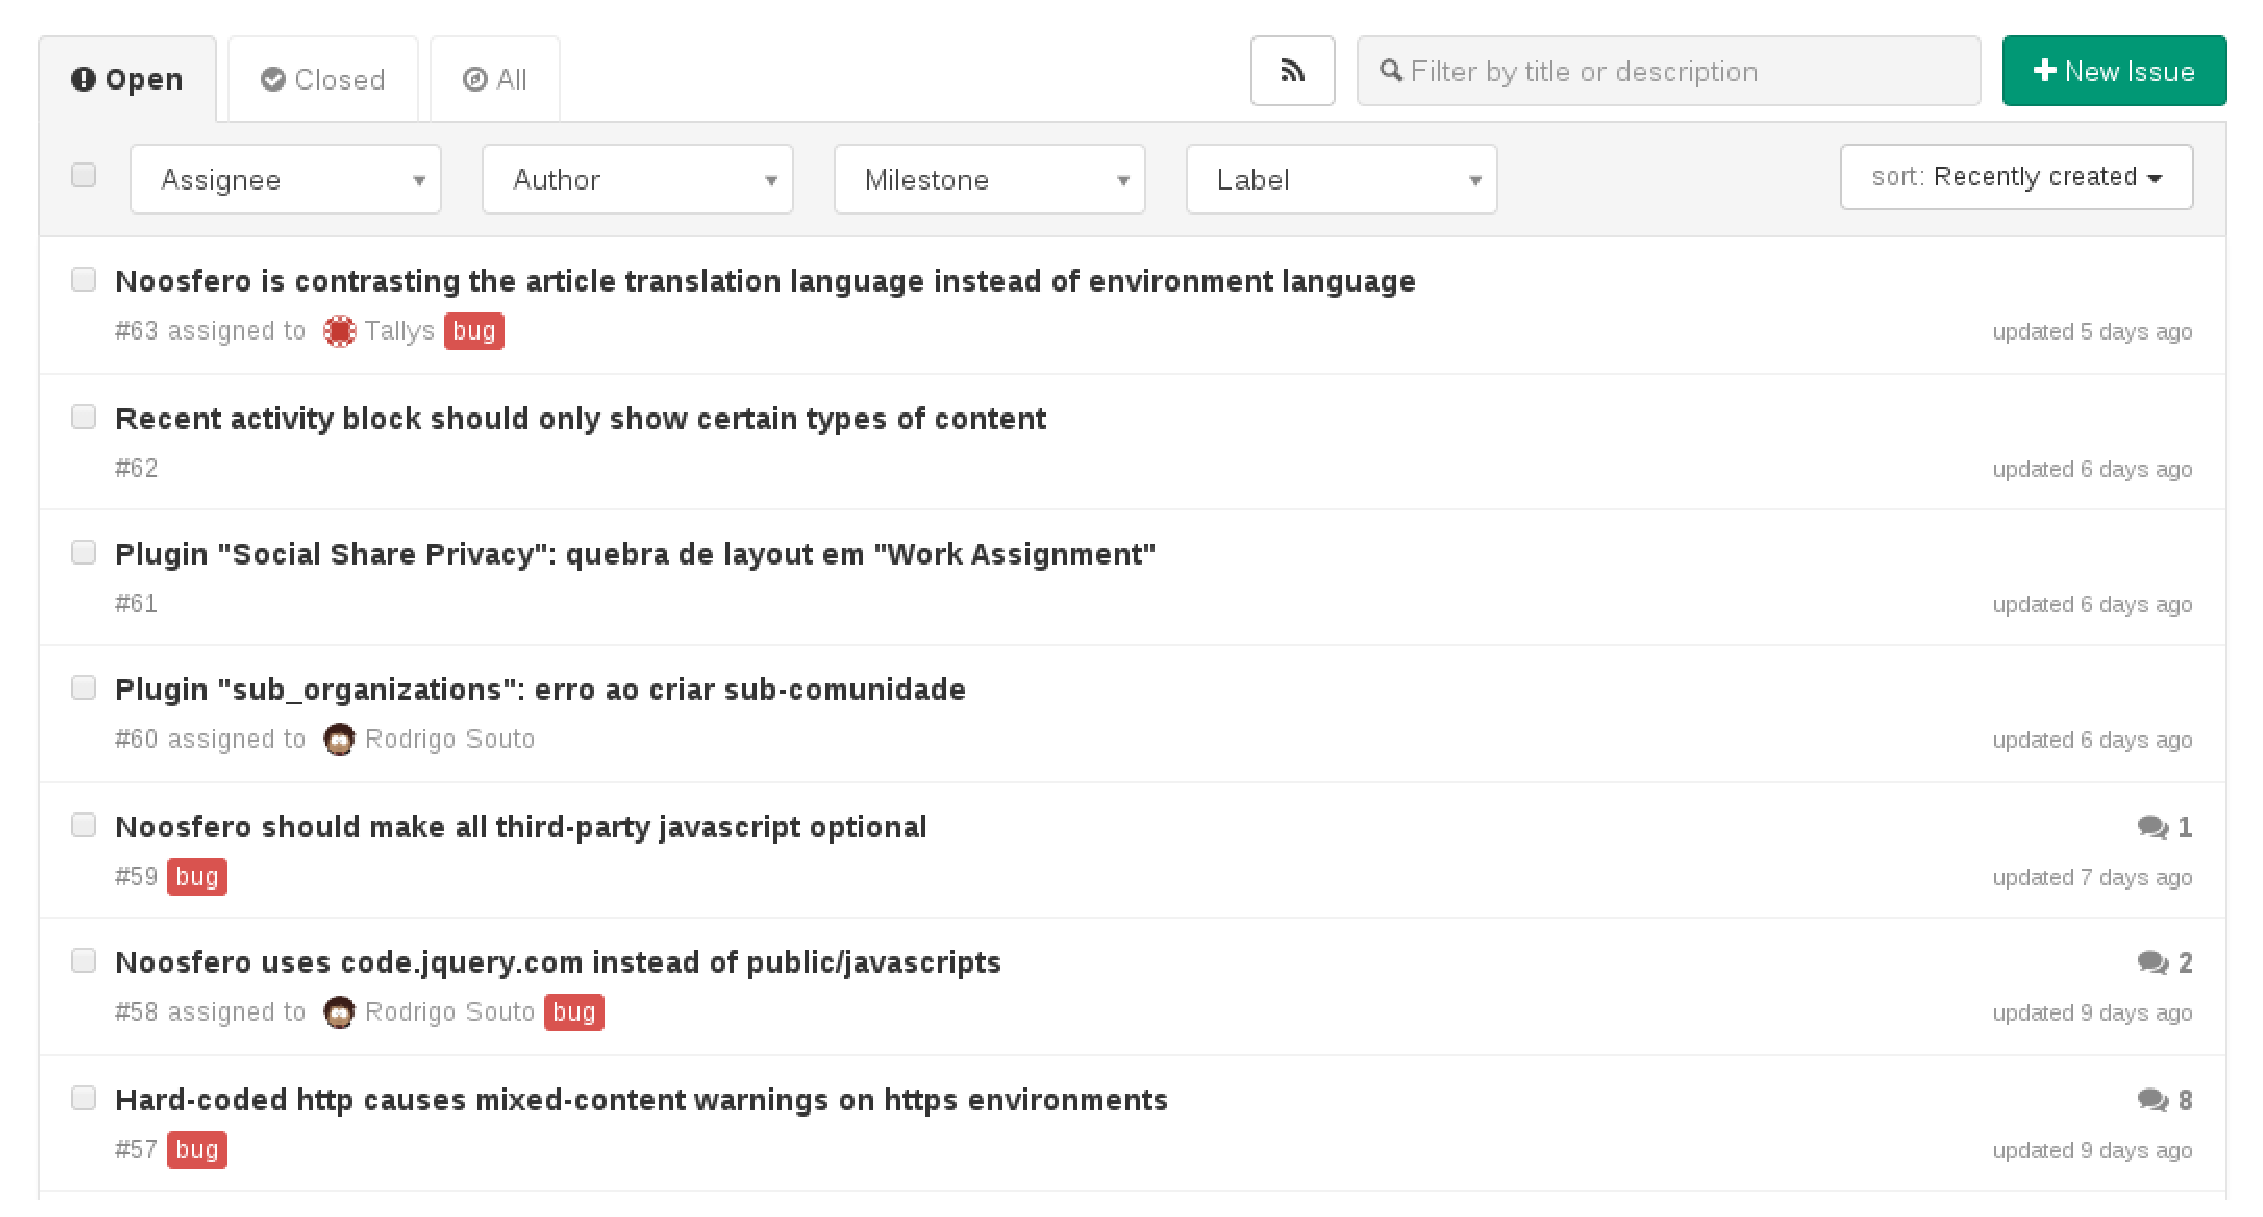
\includegraphics[keepaspectratio=true,scale=0.4]
      {figuras/issueTrackerGitLab.eps}
    \caption{Issue Tracker no GitLab}
    \label{issue-tracker}
\end{figure}

Priorizando a comunicação entre os desenvolvedores, a comunidade compartilha canais \footnote{Canais do Noosfero: \textit{\#noosfero-br} e \textit{\#noosfero}} de comunicação pelo IRC (\textit{Internet Relay Chat}). Nesses os desenvolvedores podem compartilhar conhecimento e realizarem discussões técnicas sobre as implementações.

A implementação é realizada pelo desenvolvedor que tem a responsabilidade de manter a qualidade do código produzido bem como realizar todos os testes relacionados à funcionalidade implementada. Uma vez que este primeiro passo esteja concluído o código é submetido a um \textit{merge-request} onde um dos desenvolvedores do \textit{core} efetua a revisão para verificar se está de acordo com os padrões esperados, e aprova ou não, a inclusão do código na \textit{branch} principal do Noosfero.

A comunidade Noosfero recomenda práticas de desenvolvimento como o TDD, \textit{Test Driven Development} ou Desenvolvimento orientado a testes), combinado com o BDD \footnote{\url{https://cukes.info/}} (\textit{Behavior Driven Development}) ou Desenvolvimento Guiado por Comportamento, que auxiliar o desenvolvedor a criar testes e integrar regras de negócio com a linguagem de programação, mantendo o foco no comportamento do software \cite{north2006introducing}.

Para realizar o controle de versão e gerenciamento do código fonte é utilizado o \textit{Git}, uma ferramenta livre de versionamento distribuído de código fonte. O repositório oficial do Noosfero encontra-se no software livre Gitlab com um espelho no Github\footnote{\url{https://github.com/noosfero/noosfero}}. Na página de desenvolvimento da comunidade existe uma série de recomendações sobre o envio de \textit{patches} para o Noosfero, incluindo como versionamentos e solicitações de inclusão de seu \textit{patch}, ou \textit{merge-request}.

\subsection{Arquitetura}
\label{arquitetura}

Para a evolução de um software de forma adequada é importante o conhecimento da arquitetura do sistema, para não comprometer todo o planejamento realizado na concepção do projeto. Desse modo conhecer e entender a arquitetura de funcionamento do Noosfero é uma etapa fundamental para o densevolvimento de novas funcionalidades para a plataforma.

\begin{figure}[h]
    \centering
    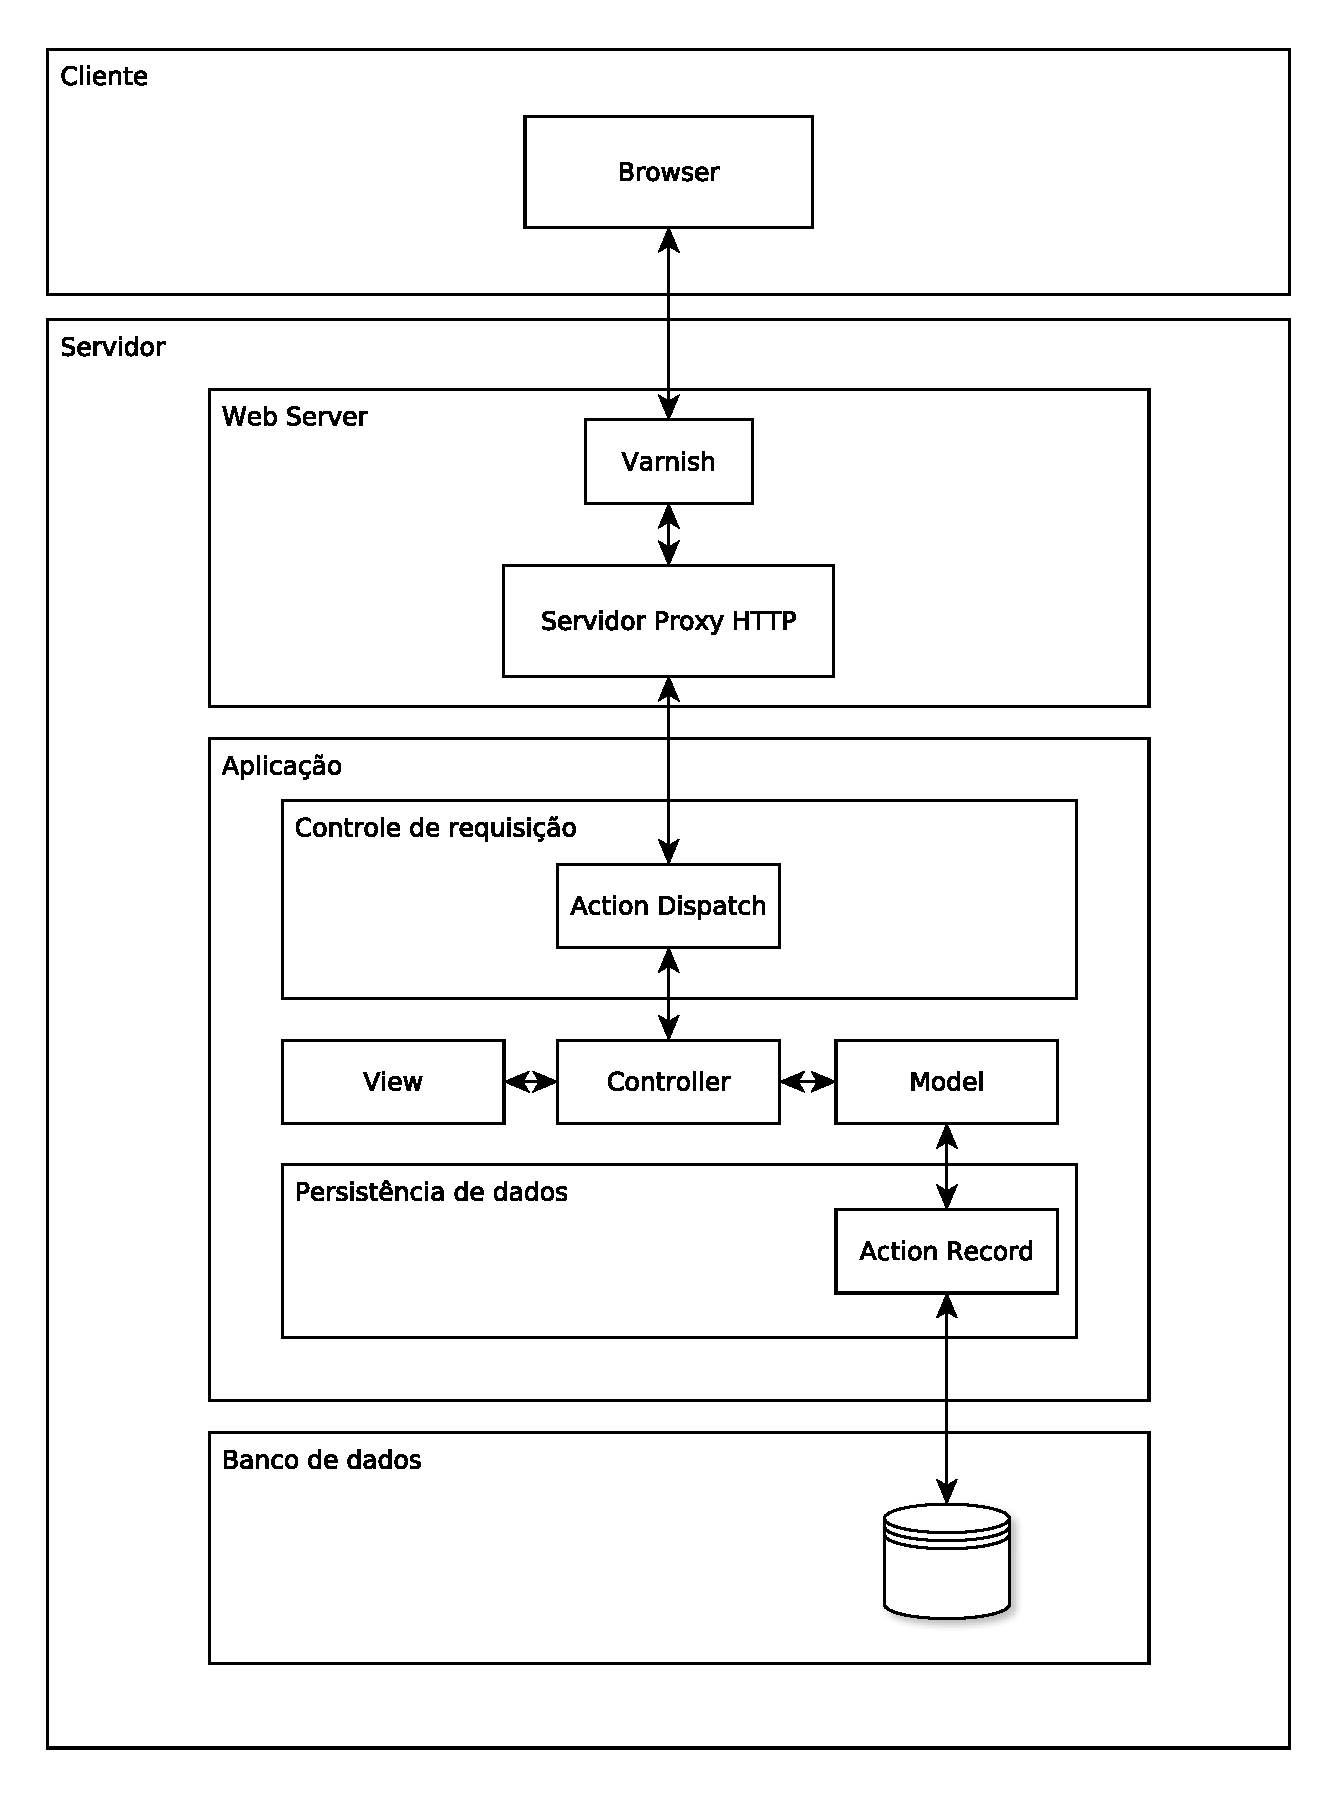
\includegraphics[keepaspectratio=true,scale=0.4]
      {figuras/DiagramaDeArquitetura.eps}
    \caption{Arquitetura do Noosfero}
    \label{arquitetura-noosfero}
\end{figure}

A Figura \ref{arquitetura-noosfero} apresenta uma visão de alto nível da arquitetura do Noofero. Basicamente tem-se uma arquitetura cliente-servidor onde o cliente via \textbf{\textit{Browser}} solicita um conteúdo ou uma função para o servidor Noosfero, que aguarda requisições de entrada para processá-las e compartilhar recursos com o cliente.

Do lado do servidor, temos basicamente três camadas de abstração: \textit{Web-Server}, \textit{aplicação} e \textit{Banco de dados}. Na primeira camada temos dois componentes responsáveis por processar e acelerar todas as requisições de entrada e saída:

\begin{itemize}
\item Varnish: é um acelerador para sites web dinâmicos com alto volume de conteúdo que utiliza \textit{proxy} HTTP Reverso. Sua efiência deve-se ao fato dele armazenar o conteúdo HTTP requisitado na memória RAM, fazendo com que o servidor não consulte e processe diversas vezes o mesmo conteúdo solicitado.
\item Servidor Proxy HTTP: pode ser utilizado o Apache ou Nginx \footnote{\url{http://nginx.org}} que ajudam a melhorar o desempenho funcionando como um servidor proxy HTTP reverso que processa as requisições de entrada e saída e as encaminha para a aplicação executá-las.
\end{itemize}

Na camada da aplicação, foi considerada uma camada responsável pelo controle de requisições, que é efetuada pelo componente \textbf{\textit{Action Dispatch}}, que lida com o mapeamento de todas as requisições, \textit{cookies} e sessão para suas respectivas \textit{controllers}.

Na aplicação, utiliza-se o padrão de arquitetura de software MVC\footnote{Model-view-controller} onde a \textbf{\textit{controller}} controla o fluxo da aplicação,relacionando as entidades de \textit{model} e de \textit{view} através de chamadas de métodos. A \textbf{\textit{model}} representa as entidades do domínio da aplicação, onde a lógica do sistema são implementadas. A \textbf{\textit{view}} é a interface de comunicação com o usuário, ou seja as páginas HTML apresentadas no navegador.

Ainda na camada da aplicação tem-se o \textbf{\textit{Active Record}} que é um ORM \footnote{object-relational mapping}, um mapeador entre objetos e registros de uma tabela, onde cada classe de modelo possui uma tabela correspondente à ela no banco de dados.

Por fim temos a camada de banco de dados que recebe requisições da camada de persistência de dados e por meio de um sistema gerenciador de banco de dados (SGBD) realizam operações na base de dados.

\subsection{Modelo de domínio}

Para \citeonline[p. 160]{larman2002utilizando}, um modelo de domínio é a representação visual de classes conceituais ou objetos do mundo real em um domínio, que também podem ser chamados de modelos conceituais, modelos de objetos de domínio e modelos de objetos de análise. Dessa forma, é necessário o seu entendimento para realizar a evolução da plataforma.

\begin{figure}[h]
    \centering
    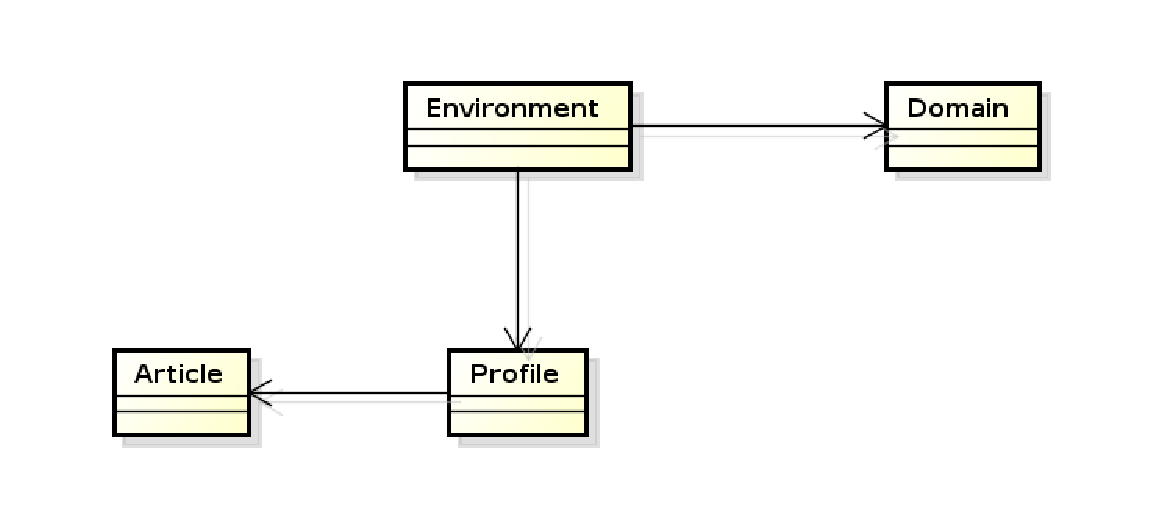
\includegraphics[keepaspectratio=true,scale=0.65]
      {figuras/domain_main.eps}
    \caption{Relações entre entidades de domínio ambiente, domínio e perfis. Extraído de: \cite{bucher2013rede}}
    \label{domain_main}
\end{figure}

O Noosfero é uma plataforma que tem suporte a vários ambientes de rede social dentro de uma mesma instalação. A Figura \ref{domain_main} mostra-se o funcionamento geral do Noosfero com suas quatro principais classes \textbf{\textit{Domain}}, \textbf{\textit{Environment}}, \textbf{\textit{Profile}} e \textbf{\textit{Article}} (Em português: Domínio, Ambiente, Perfil e Artigo respectivamente). Analisando o modelo verifica-se que na implementação é necessário que exista pelo um domínio e partir disso é possível criar várias instâncias de Ambiente na aplicação.

\begin{figure}[h]
    \centering
    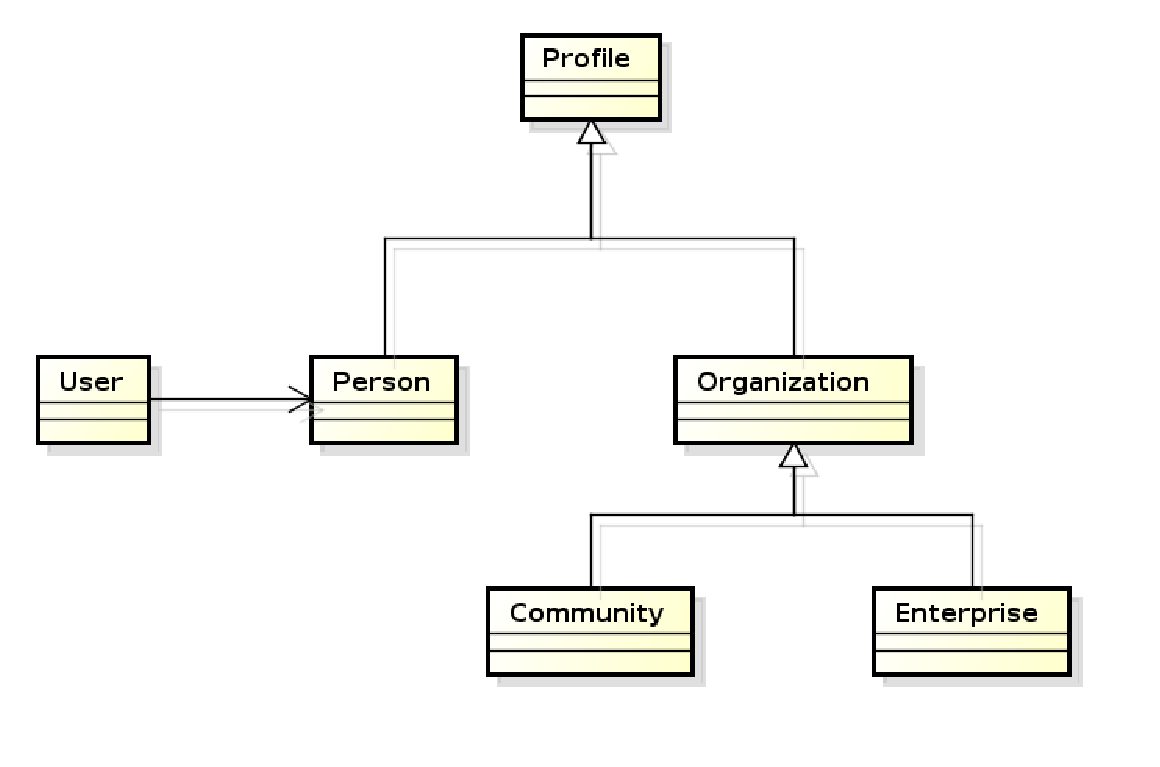
\includegraphics[keepaspectratio=true,scale=0.6]
      {figuras/domain_profiles.eps}
    \caption{Entidades de domínio: tipos de perfis. Extraído de: \cite{bucher2013rede}}
    \label{domain_profiles}
\end{figure}

A entidade Profile é uma generalização das entidades \textbf{\textit{Person}} (Pessoa) e \textbf{\textit{Organization}} (Organização), como pode ser visto na Figura \ref{domain_profiles}. Nesse mesmo modelo percebe-se que Organization é especializada nas entidades concretas \textbf{\textit{Community}} (Comunidade e Enterprise (Empreendimento). A herança é um mecanismo pelo qual qual uma classe sub-classe pode estender uma super-classe, onde basicamente isola-se métodos ou atributos em comum dentro de uma classe pai (super-classe), enquanto as especialidades são responsabilidade das classes filhas (sub-classe).

Por questões de design do código da aplicação foi criada uma entidade \textbf{\textit{User}}, ou Usuário, que é mantida separada da entidade Pessoa, que é quem implementa a lógica de autenticação da aplicação. Desta forma a lógica de autenticação fica separada da lógica de visualização e personalização do perfil.

\begin{figure}[h]
    \centering
    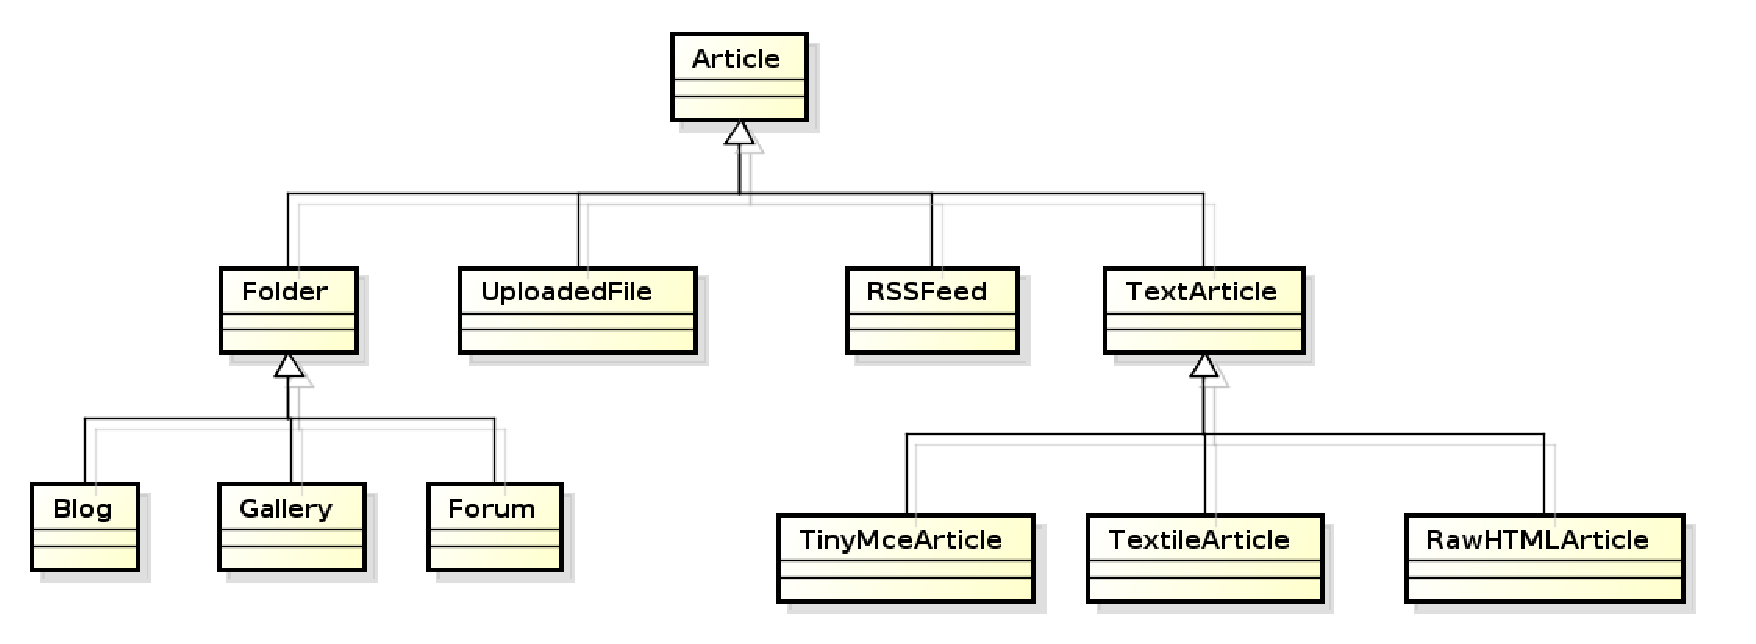
\includegraphics[keepaspectratio=true,scale=0.55]
      {figuras/domain_articles.eps}
    \caption{Entidades de domínio: tipos de artigos. Extraído de: \cite{bucher2013rede}}
    \label{domain_articles}
\end{figure}

Por fim, as entidades mostradas na Figura \ref{domain_articles} representam os principais tipos de conteúdos disponíveis no Noosfero, onde a classe \textbf{\textit{Article}}, ou Artigo, é uma especialização de todos os conteúdos disponíveis como: artigos de texto, pastas, blogs, galerias de imagens, fórum, arquivos e feeds de notícias.

O modelo de domínio aqui apresentado contempla o \textit{core} do noosfero. Para o acréscimo de melhorias e funcionalidades é necessário compreender a visão arquitetural dos \textit{plugins} d a plataforma, que será abordado na próxima seção.

\subsection{Plugins}
\label{plugins-noosfero}

Como é software em constante evolução, a arquitetura do Noosfero foi criada para ser altamente expansível, fazendo-se o uso de \textit{plugins}. Essa arquitetura permite que em cada ambiente fique a critério do usuário quais os \textit{plugins} ou novas funcionalidades serão habilitadas, o que torna o sistema flexível e modular.

% Aumentar figura 6
\begin{figure}[h]
    \centering
    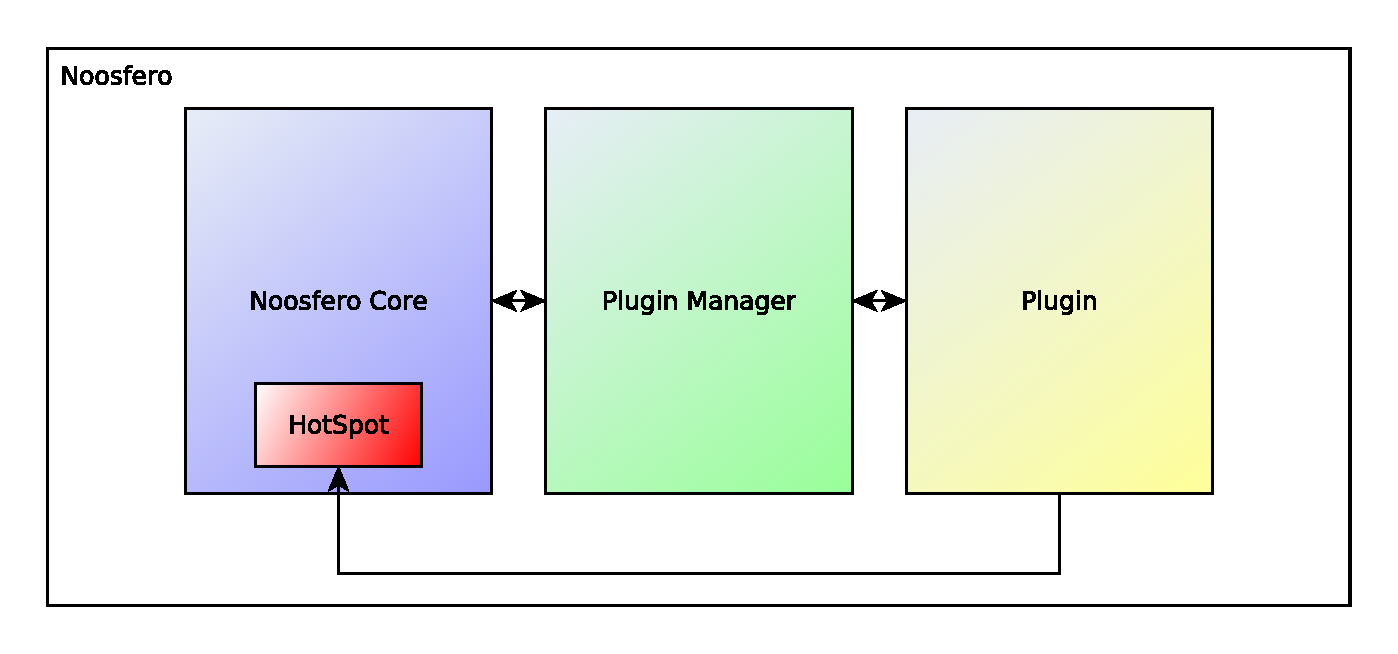
\includegraphics[keepaspectratio=true,scale=0.7]
      {figuras/estruturaDePlugins.eps}
    \caption{Estrutura de Plugins}
    \label{estrutura-plugins}
\end{figure}

A Figura \ref{estrutura-plugins} é uma abstração alto nível do funcionamento interno dos plugins no Noosfero. No \textit{core} do Noosfero temos os \textit{hotspots}, que são pontos de flexibilidade que permitem associar diferentes comportamentos na execução do sistema, permitindo a inserção de trechos de código e ou alteração de um determinado método sem comprometer suas funcionalidades básicas.

Os \textit{hotspots} são gerenciados por uma camada de abstração denominada \textit{Plugin Manager}, ou Gerenciador de \textit{Plugins}, que são chamadas pelo \textit{core} através de um metódo principal conhecido como \textit{dispatch}. Basicamente, o ciclo de execução pode ser descrito da seguinte maneira: durante a execução de alguma funcionalidade o método \textit{dispatch} é invocado por alguma funcionalildade do core, deste modo o gerenciador de plugins verifica todos os \textit{Plugins} que fazem uso daquele \textit{hotspot} e encaminha para cada um deles a execução de suas ações de acordo com sua implementação.

Essa arquitetura extensível adotada pelo Noosfero auxilia no controle da qualidade de código das novas funcionalidades. A camada de \textit{Plugins} localiza-se fora do código do seu núcleo, em uma pasta denominada \textit{plugins} em que desenvolvedor cria novas funcionalidades sem modificar o comportamento \textit{core} do Noosfero, fazendo uso dos \textit{dispatch}.

Adicionalmente como mencionado na Seção \ref{proc-desenvol-comunidade}, o Noosfero faz uso de testes para manter a integridade de seu código, desse modo esta prática é estendida aos \textit{plugins} que devem englobar seus respectivos testes para evitar a inserção de \textit{bugs} e mudanças inesperadas no comportamento do sistema. 

Assim sendo a evolução proposta para este trabalho será realizada através de plugins, como proposto na Seção \ref{desen-noosferAVA}

\section{Comunidade UnB}
\label{comunidade-unb}

A Comunidade.UnB é uma rede colaboração livre desenvolvida para que alunos, professores e servidores técnico-administrativos tenham um ambiente virtual de criação e compartilhamento de conhecimento colaborativo. É um ambiente virtual para o compartilhamento de ideias, produção de conteúdo colaborativo de modo que possam publicá-los para que possa ser de utilidade para outras pessoas ou parcelas da sociedade, uma vez que acredita-se que este é um dos papéis de uma Universidade \cite{bucher2013rede}.

\begin{figure}[!htb]
    \centering
    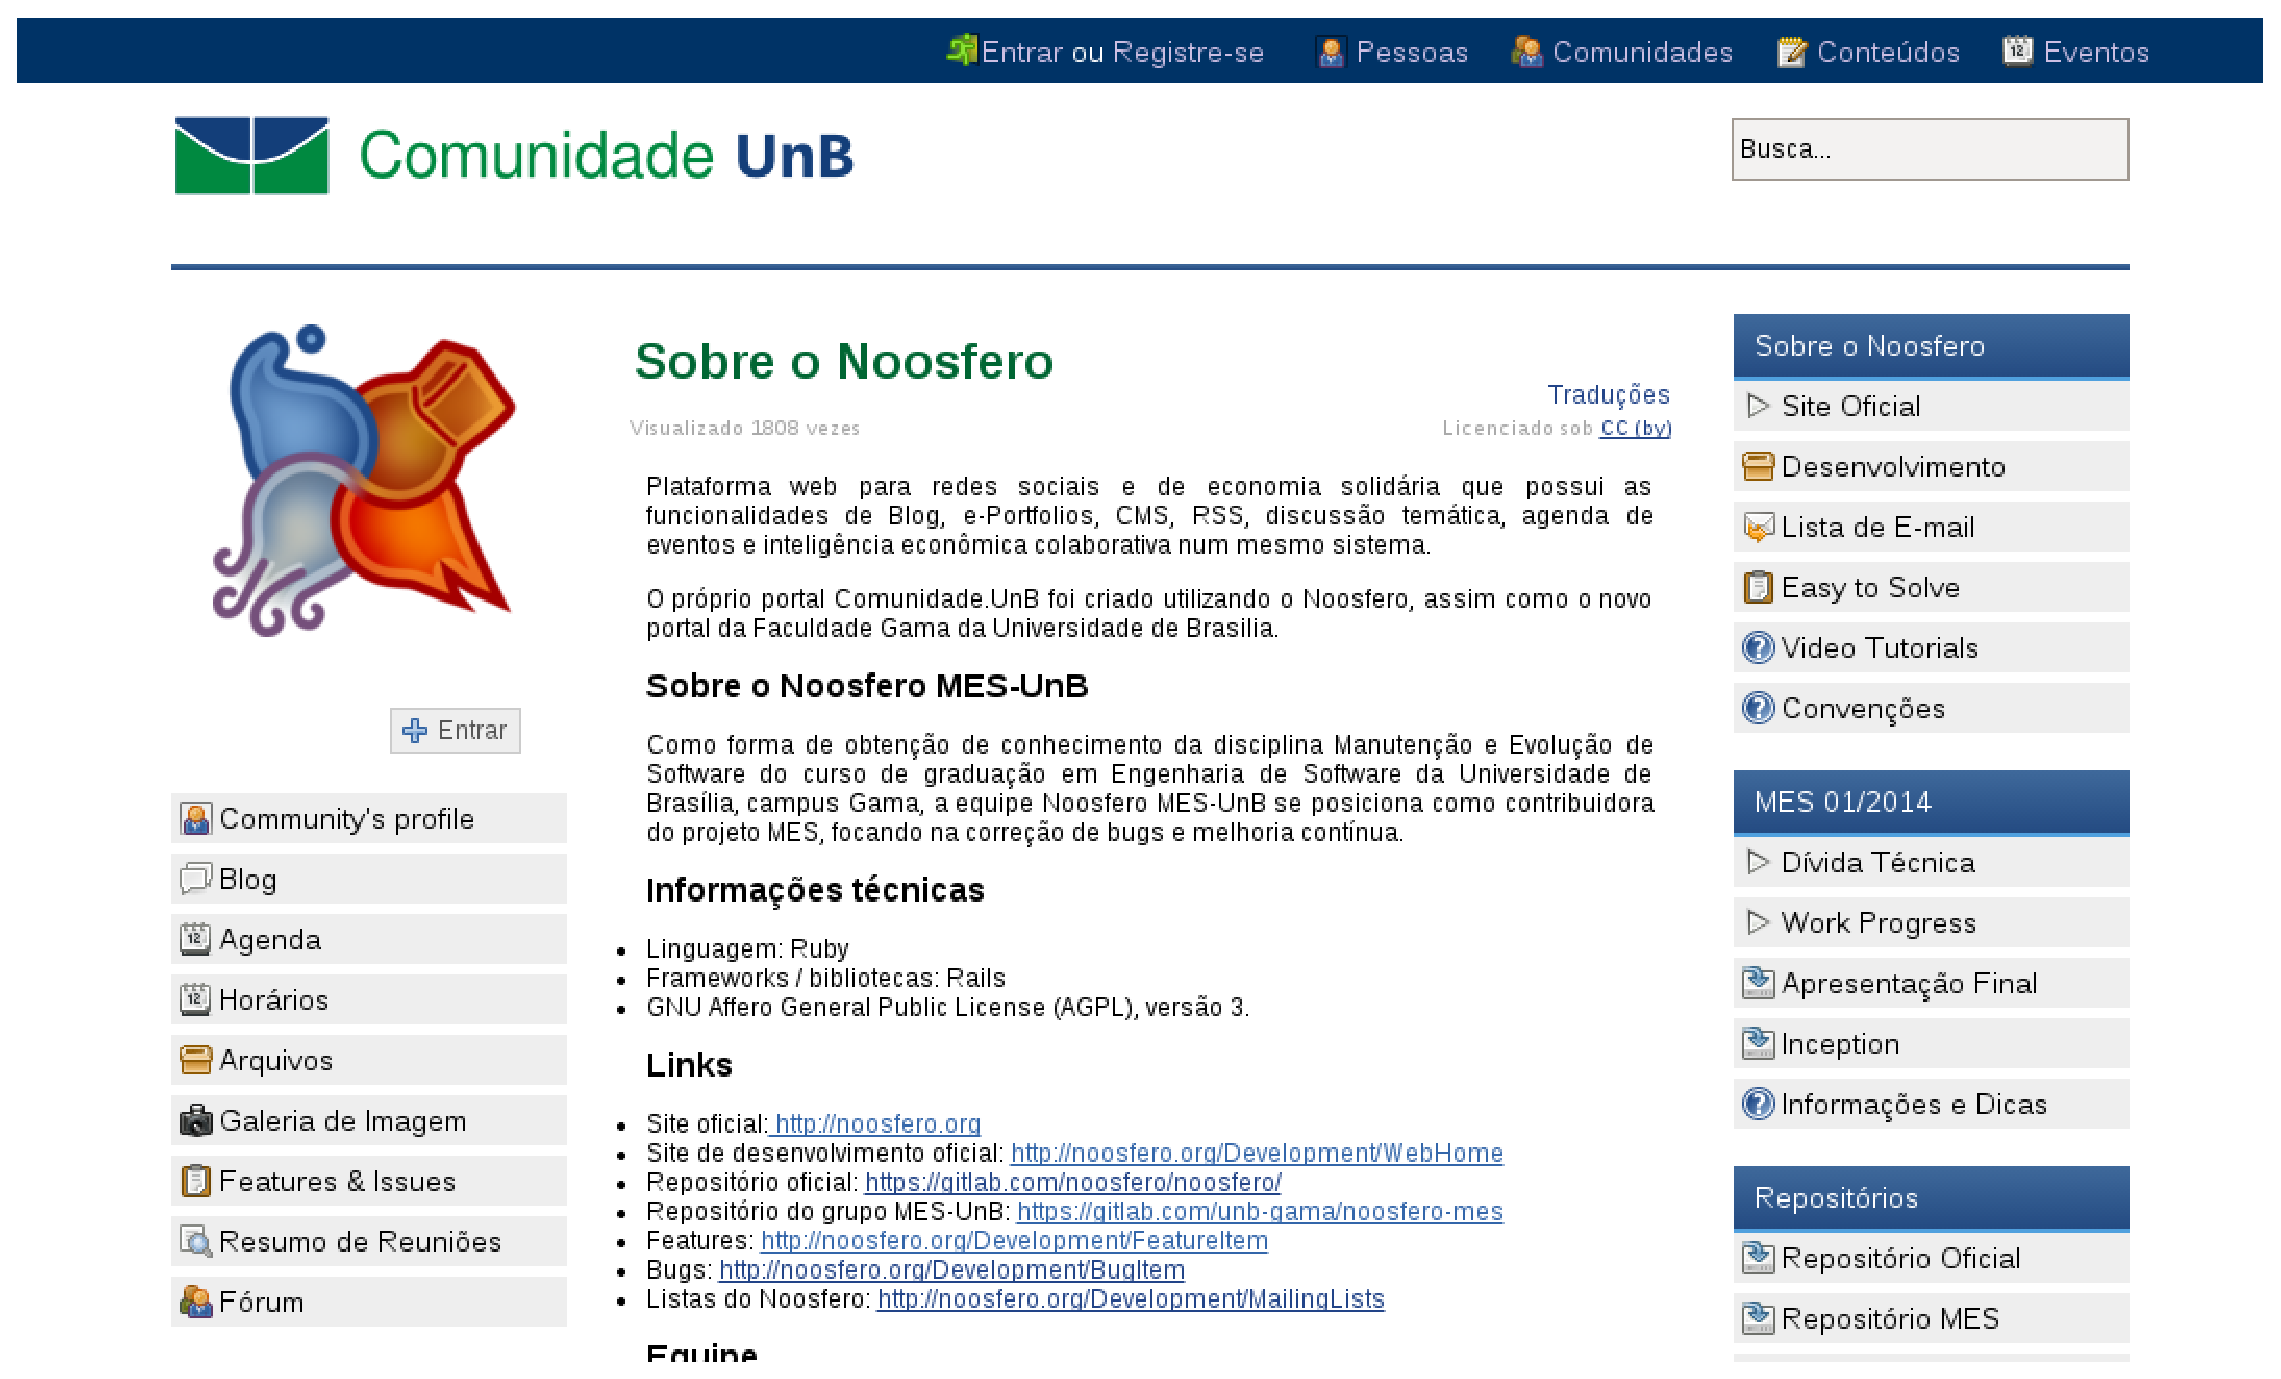
\includegraphics[keepaspectratio=true,scale=0.4]
      {figuras/comunidade-mes.eps}
    \caption{Exemplo do uso do Comunidade.UnB na disciplina de MES.}
    \label{comunidade-mes}
\end{figure}

Inspirada na rede social de colaboração Stoa \footnote{Disponível em: \url{https://social.stoa.usp.br/}}, da Universidade de São Paulo (USP), a Comunidade.UnB foi criada em 2013 a partir de um trabalho de conclusão de curso de Daniel Costa Bucher e até então está disponibilizada em ambiente de testes. Permite ao usuário a criação de seu espaço pessoal e a liberdade de publicar suas ideias, ou o conteúdo que desejar, por exemplo, na forma de blogs pessoais, blogs de disciplinas, pesquisas em andamento, dentre outras, além de compartilhar esse conteúdo para ser acessível para outros usuários dentro e fora da rede.

O Noosfero, descrito na Seção \ref{noosfero}, foi a plataforma utilizada para o desenvolvimento da Comunidade.UnB, por dispor de um grande potencial e devido às suas funcionalidades avançadas, que permitem a criação e o compartilhamento de conteúdo de forma satisfatória. Além de dispor de uma comunidade ativa e de posição geográfica favorável em relação ao seu núcle de desenvolvimento que se encontra no Brasil, facilitando a comunicação com os seus principais desenvolvedores.

Apesar da Comunidade.UnB estar disponibilizada como um ambiente de testes e não possuir uma vasta divulgação pela Universidade de Brasília, no seu primeiro ano de criação contava com 153 usuários e 14 comunidades. Ao final de maio de 2015 contabilizava 376 usuários e 30 comunidades demonstrando que houve crescimento.

Alguns professores adotaram a Comunidade.UnB como um ambiente de apoio ao Moodle, AVA oficial adotado pela UnB. Na Figura \ref{comunidade-mes} é apresentado um exemplo de seu uso na disciplina de Manutenção e Evolução de Software (MES) ministrada pelo professor Paulo Roberto Miranda Meirelles.

Esse é um exemplo de comunidade criada dentro do Comunidade.UnB, que possui características que se assemelham ao ambiente Moodle, como evidenciado na Seção \ref{comparacao-ava}, carece de alguns funcionalidades importantes mas com a vantagem da possibilidade de acesso do público ao conteúdo, e a continuidade do conteúdo desenvolvido por outras pessoas que eventualmente se juntem ao longo do tempo. Vale lembrar que em uma publicação de conteúdo os níveis de privacidade podem ser alterados basicamente entre públicos e privados.

As limitações da plataforma e a proposta de uso da Comunidade.UnB por professores para a criação de disciplinas, estimulam o desenvolvimento de funcionalidades que levem à plataforma Noosfero a assemelhar-se a um ambiente virtual de aprendizagem. Dessa maneira na Seção \ref{desen-noosferAVA} é apresentada a proposta de estudo desse trabalho para desenvolvimento de funcionalidades e minimização das diferenças entre o Noosfero e os ambientes virtuais de aprendizegem.

\section{Desenvolvimento do NoosferAVA}
\label{desen-noosferAVA}

Nesta seção apresentaremos as funcionalidades que serão desenvolvidas para contribuir para a adequação do Noosfero a um ambiente virtual de aprendizagem, para exercer a função de apoio aos AVA adotados pela universidade. Serão apresentados os requisitos funcionais levantados para que esta possa suprir as necessidades levantadas.

Além das funcionalidades relatadas, julgou-se necessária a evolução do \textit{plugin Comunidade.UnB}, iniciado por \citeonline{bucher2013rede}, com objetivo de integrar o Noosfero com o serviço de Lightweight Directory Access Protocol (LDAP). Uma base LDAP é utilizada pela UnB para manter os dados de todos os seus alunos e funcionários.

As funcionalidades serão apresentadas utilizando o formato de histórias de usuários \footnote{Em inglês \textit{User Stories}(US)}, de acordo com as práticas ágeis. Além disso, os critérios de aceitação serão expostos no formato de cenários de uso, utilizando BDD.

\subsection{Evolução do \textit{plugin Comunidade.UnB}}
\label{plugin-comunidade}

O objetivo do \textit{plugin} do Comunidade.Unb é que o usuário tenha acesso através dos mesmos dados utilizados para acessar outros serviços, como, por exemplo, o serviço de matrícula \footnote{Disponível em: \url{https://matriculaweb.unb.br}} para alunos ou o serviço de lançamento de notas para professores.

A versão anterior do \textit{plugin} permitia que apenas os novos usuários realizassem o cadastro de suas matrículas, dessa maneira aqueles que já estavam cadastrados não tinham acesso ao portal. Devido às limitações de acesso definidas pelo \textit{plugin}, onde apenas usuários com matrícula cadastrada tem acesso ao sistema.

Foi criada nova versão do \textit{plugin} que permite cadastrar a matrícula dos usuários que já possuem registro no Comunidade.UnB. Dessa maneira, o \textit{plugin Comunidade.UnB} poderá ser ativado permitindo a autenticação apenas dos usuários cadastrados no LDAP da universidade. Abaixo segue a história de usuário com seus respectivos cenários de uso.

\subsubsection*{Histórias de usuário}

% história
\begin{enumerate}
\item \underline{Autenticação via LDAP}

\textbf{Como} um aluno da Universidade Brasília

\textbf{Gostaria de} me autenticar na rede através da minha matrícula e senha

\textbf{Para} utilizar os mesmos dados de cadastro da UnB.

\subsubsection*{Cenários de uso:}

% cenário
\begin{enumerate}
\item \underline{Acesso sem matrícula cadastrada}

\textbf{[Dado]} que sou aluno da UnB

\textbf{[E]} possuo cadastro ativo na base de dados da UnB

\textbf{[E]} possuo cadastro ativo na base de dados do Comunidade.UnB

\textbf{[Quando]} eu acessar o portal

\textbf{Como} um aluno da Universidade Brasília

\textbf{[Então]} devo ser direcionado para uma página com o título ``Cadastrar Matrícula''

\textbf{[E]} devo ver os campos ``Matrícula'', ``Senha'' e
``confirmação de senha'' em branco.

\item \underline{Registro de matrícula de usuários existentes}

\textbf{[Dado]} que sou aluno da UnB

\textbf{[E]} me encontro na página de Cadastrar matrícula do Comunidade.UnB

\textbf{[Quando]} eu preencher os campos \\
``matrícula'' com ``100103979'',\\
e ``senha''  com a senha da base dados da UnB,\\
e ``confirmação de senha''

\textbf{[E]} clicar no botão ``Registrar''

\textbf{[Então]} eu devo ser direcionado para meu perfil
% cenários
\end{enumerate}
% histórias
\end{enumerate}

% -------------------- Evolução do Work Assignment ----------------
\subsection{Evolução do \textit{plugin Work Assignment}}

Nesta subseção serão apresentadas um primeiro levantamento das histórias correspondentes a evolução do \textit{plugin Work Assignment}. Até então, o \textit{plugin} possui apenas a funcionalidade de permitir o envio de arquivos para o servidor em um determinado período de tempo.

A proposta de evolução é a criação de um sistema de notas que permita ao professor atribuir notas as atividades enviadas e dessa maneira acompanhar a situação de cada aluno. Do ponto de vista do aluno, o mesmo poderá visualizar todas as notas das atividades em cada disciplina, avaliando se o seu desempenho está satisfatório.

Além disso, é necessário uma evolução da funcionalidade que permite a definição do tempo restante para o envio, que atualmente é realizado de maneira manual, não possibilitando o estabelecimento de intervalos de tempo.

\subsubsection*{Histórias de usuário}
% história
\begin{enumerate}
% ---------------------------------------------------------------------
\item \underline{Definir tempo restante}

\textbf{Como} um professor

\textbf{Gostaria de} definir o tempo restante para cada atividade no Work Assignment

\textbf{Para} gerenciar o envio de atividades pelos alunos em um determinado período.

\subsubsection*{Cenários de uso:}

\begin{enumerate}
\item \underline{Definir tempo}

\textbf{[Dado]} que esteja logado como professor

\textbf{[E]} selecione a o opção ``Gerenciar conteúdo''

\textbf{[Quando]} eu clicar em trabalho a ser entregue

\textbf{[Então]} devo visualizar a opção ``Ativar tempo de entrega''

\textbf{[E]} informar a data e hora máxima para envio da atividade.

\item \underline{Modificar tempo}

\textbf{[Dado]} que esteja logado como professor

\textbf{[E]} eu tenha atividades a ser entregue em aberto

\textbf{[E]} eu esteja visualizando as informações da atividade

\textbf{[Quando]} eu selecionar opção ``Editar''

\textbf{[E]} visualizar a opção ``Tempo de entrega''

\textbf{[Então]} deve ser permitido que eu altere o tempo definido

\textbf{[E]} visualize o resultado da alteração após a confirmação.

\item \underline{Permitir entrega de atividades após período}

\textbf{[Dado]} que esteja logado como professor

\textbf{[E]} selecione a o opção ``Gerenciar conteúdo''

\textbf{[E]} vavegar até a página trabalho a ser entregue

\textbf{[Quando]} selecionar a opção ``Ativar tempo de entrega''

\textbf{[Então]} devo visualizar a opção ``Permitir entrega após o período''

\textbf{[Para]} que eu possa selecioná-la.

\end{enumerate}
% -----------------------------------------------------------------------
\item \underline{Tempo restante de atividades}

\textbf{Como} um aluno

\textbf{Gostaria de} visualizar o tempo restante da atividade

\textbf{Para} enviar um arquivo na data correta.

\subsubsection*{Cenários de uso:}

\begin{enumerate}
\item \underline{Visualizar tempo}

\textbf{[Dado]} que esteja logado como Aluno

\textbf{[E]} eu esteja inscrito em um Curso

\textbf{[E possua atividade em aberto]}

\textbf{[Quando]} eu selecionar a opção de visualizar a atividade

\textbf{[Então]} eu devo visualizar se a atividade está em aberto

\textbf{[E]} qual o tempo restante para o envio da atividade.

\end{enumerate}

% -----------------------------------------------------------------------
\item \underline{Professor gerencia notas}

\textbf{Como} um professor

\textbf{Gostaria de} gerenciar as notas dos integrantes da comunidade

\textbf{Para} manter o controle sobre a pontuação de todos os alunos.

\subsubsection*{Cenários de uso:}

\begin{enumerate}

\item \underline{Definir grupo de atividades}

\textbf{[Dado]} que esteja logado como professor

\textbf{[E]} que a funcionalidade de notas eteja habilitada no plugin

\textbf{[E]} selecionar a opção ``Gerenciar notas''

\textbf{[E]} e eu selecionar o curso desejado

\textbf{[Quando]} eu clicar em ``Cadastrar grupo de atividades''

\textbf{[E]} eu preencho os campos \\
``Nome do grupo'',\\
e ``Lista de Atividades''\\
\textbf{[E]} eu clico em ``Salvar''

\textbf{[Então]} recebo uma mensagem de confirmação

\textbf{[E]} visualizo todas os grupos de atividades criados.

\item \underline{Visualizar notas de todos os alunos de uma determinada atividade}

\textbf{[Dado]} que esteja logado como professor

\textbf{[E]} que a funcionalidade de notas eteja habilitada no plugin

\textbf{[E]} selecionar a opção ``Gerenciar notas''

\textbf{[E]} e eu selecionar o curso desejado

\textbf{[Quando]} eu selecionar atividade

\textbf{[E]} algum aluno tenha enviado a atividade

\textbf{[Então]} devo visualizar todas as atvidades enviadas e suas respectivas notas.

\item \underline{Visualizar notas de todos ao alunos de um grupo de atividades}

\textbf{[Dado]} que esteja logado como professor

\textbf{[E]} que a funcionalidade de notas eteja habilitada no plugin

\textbf{[E]} selecionar a opção ``Gerenciar notas''

\textbf{[E]} e eu selecionar o curso desejado

\textbf{[Quando]} eu clicar em ``Visualizar notas por grupo de atividades''

\textbf{[E]} algum aluno tenha enviado a atividade

\textbf{[Então]} devo visualizar todas as atvidades daquele grupo e suas respectivas notas.

\end{enumerate}
% -----------------------------------------------------------------------

\item \underline{Atribuir notas aos alunos}

\textbf{Como} um professor

\textbf{Gostaria de} atribuir notas as atividades enviadas pelos alunos

\textbf{Para} avaliar o rendimento de cada um deles.

\subsubsection*{Cenários de uso:}

\begin{enumerate}
\item \underline{Atribuir notas}

\textbf{[Dado]} que esteja logado como professor

\textbf{[E]} que a funcionalidade de notas eteja habilitada no plugin

\textbf{[Quando]} selecionar uma atividade na lista de atividades

\textbf{[Então]} devo visualizar a opção atribuir nota

\textbf{[E]} devo visualizar o campo ``nota'' para preenche-lo.


\item \underline{Alterar notas}

\textbf{[Dado]} que esteja logado como professor

\textbf{[E]} que a funcionalidade de notas eteja habilitada no plugin

\textbf{[Quando]} selecionar uma atividade na lista de atividades

\textbf{[E]} atividade já possua notas

\textbf{[Então]} devo visualizar a opção alterar nota

\textbf{[E]} devo visualizar o campo ``nota'' para preenche-lo.

\end{enumerate}

% -----------------------------------------------------------------------

\item \underline{Publicar notas aos alunos}

\textbf{Como} um professor

\textbf{Gostaria de} publicar as notas atribuídas as atividades

\textbf{Para} que os alunos possam visualizar suas respectivas avalizações

\subsubsection*{Cenários de uso:}

\begin{enumerate}
\item \underline{Disponibilizar notas de uma determinada atividade}

\textbf{[Dado]} que esteja logado como professor

\textbf{[E]} que a funcionalidade de notas eteja habilitada no plugin

\textbf{[Quando]} selecionar uma atividade na lista de atividades

\textbf{[Então]} devo visualizar a opção ``permitir visualização''

\textbf{[E]} devo ter a opção de ativá-lo.

\item \underline{Omitir notas de uma determinada atividade}

\textbf{[Dado]} que esteja logado como professor

\textbf{[E]} que a funcionalidade de notas eteja habilitada no plugin

\textbf{[Quando]} selecionar uma atividade na lista de atividades

\textbf{[Então]} devo visualizar a opção ``permitir visualização''

\textbf{[E]} devo ter a opção de desativá-lo.

\end{enumerate}

% -----------------------------------------------------------------------
\item \underline{Aluno visualiza notas}

\textbf{Como} um aluno

\textbf{Gostaria de} visualizar minhas notas

\textbf{Para} inteira-me sobre minha pontuação nas atividades.

\subsubsection*{Cenários de uso:}
\begin{enumerate}

\item \underline{Visualizar cursos com notas disponíveis}

\textbf{[Dado]} que estou logado como ``Hebert''

\textbf{[E]} o plugin Work Assignment esteja ativo

\textbf{[E]} participo de alguma comunidade que utilize o plugin de notas

\textbf{[E]} existem notas de atividades disponíveis

\textbf{[E]} o professor tenha permitido sua visualização

\textbf{[Quando]} eu navegar até a página ``Minhas notas''

\textbf{[Então]} tenho que ver todos as comunidades (cursos) com notas disponíveis.

\item \underline{Detalhar notas de cada curso}

\textbf{[Dado]} que estou logado como ``Hebert''

\textbf{[E]} o plugin Work Assignment esteja ativo

\textbf{[E]} participo de alguma comunidade que utilize o plugin de notas

\textbf{[E]} existem notas de atividades disponíveis

\textbf{[E]} o professor tenha permitido sua visualização

\textbf{[E]} navegar até a página ``Minhas notas''

\textbf{[E]} visualizar todos as comunidades (cursos) com notas disponíveis

\textbf{[Quando]} eu selecionar a ``Visualizar detalhes'' de alguma comunidade

\textbf{[Então]} tenho que ver todos os grupos de atividades

\textbf{[E]} as notas disponibilizadas pelo professor.
% cenários
\end{enumerate}
% historia
\end{enumerate}

No contexto da UnB, o desenvolvimento dessa funcionalidade é importante, pois segundo o documento da instituição \citeonline[p. 37]{unb-professor}, as notas para os alunos auxilia assimilação progressiva de conhecimento, e sabe-se que permite um maior \textit{feedback} para o aluno, pois nem sempre fica transparente o seu desempenho ao longo do semestre.

Em resumo, as funcionalidades apresentadas neste capítulo irão colaborar para uso do Comunidade.UnB, tornando-o uma plataforma híbrida entre um ambiente virtual de aprendizagem e uma rede social, para a troca de conhecimento através das comunidades e perfis de usuários. Assim, permitindo englobar departamentos, organizações e projetos específicos da Universidade de Brasília.


\chapter{O Desenvolvimento}
\label{consideracoes-preliminares}

A partir dos requisitos levantados e levando em consideração as práticas ágeis utilizadas no LAPPIS foram realizadas \textit{sprints} com duração de quinze dias. Em cada uma dessas foram desenvolvidas histórias de acordo com a pontuação e demanda de atividades na equipe do Portal, visto que o desenvolvimento foi realizado de maneira colaborativa.

\begin{figure}[h]
    \centering
    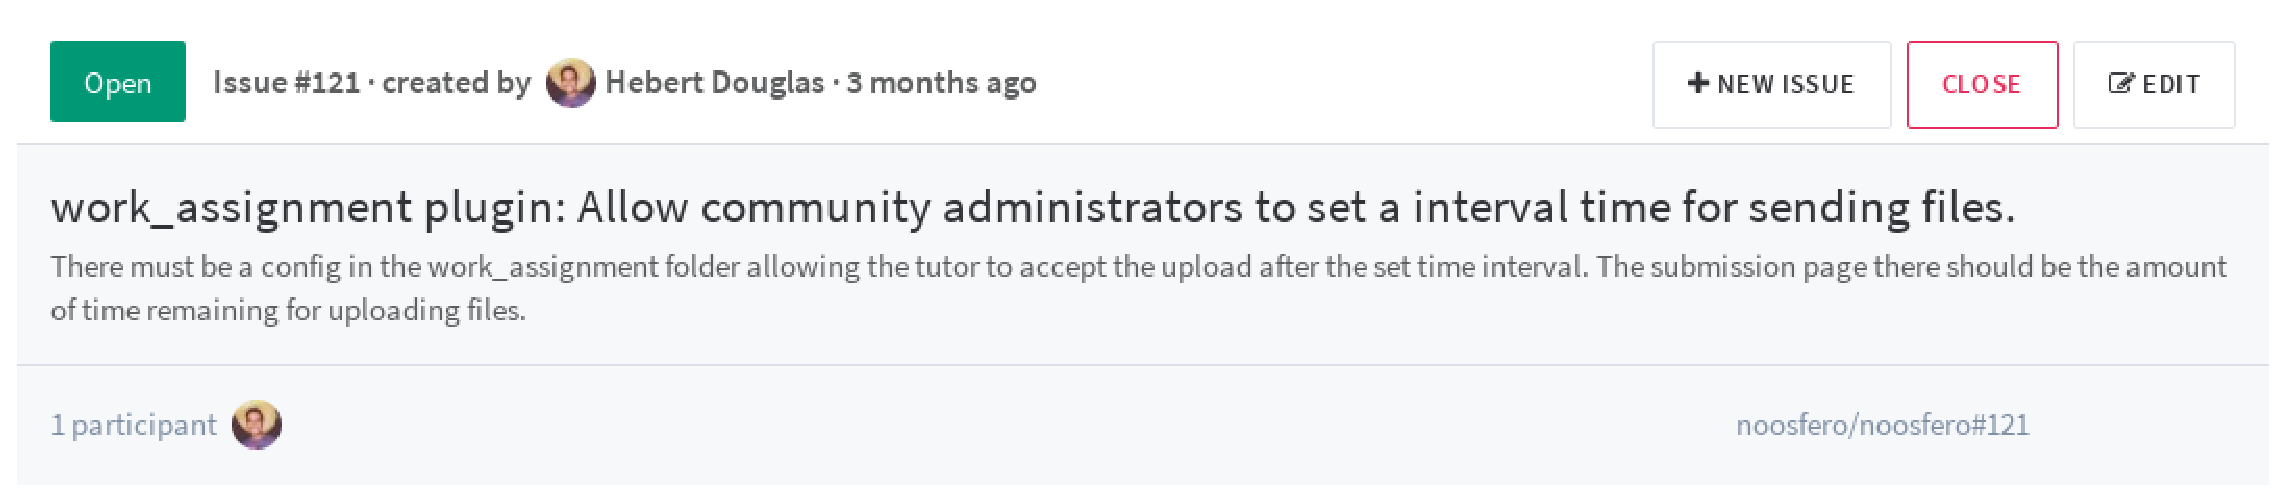
\includegraphics[keepaspectratio=true,scale=0.4]
      {figuras/issue121.eps}
    \caption{Issue 121: Gerenciamento de tempo para work\_assignment}
    \label{fig:issue-121}
\end{figure}

A primeira \textit{sprint} de desenvolvimento das histórias de usuário, foi iniciada em Julho junto com a equipe do Portal FGA. Seguindo as práticas de desenvolvimento da comunidade Noosfero, criou-se uma \textit{Issue} para evidenciar aos desenvolvedores o ínicio da implementação de uma nova funcionalidade. A \textit{Issue} criada foi a de número 121\footnote{Disponível em: \url{https://gitlab.com/noosfero/noosfero/issues/121}} que  é evidenciada na Figura \ref{fig:issue-121}

\begin{figure}[h]
    \centering
    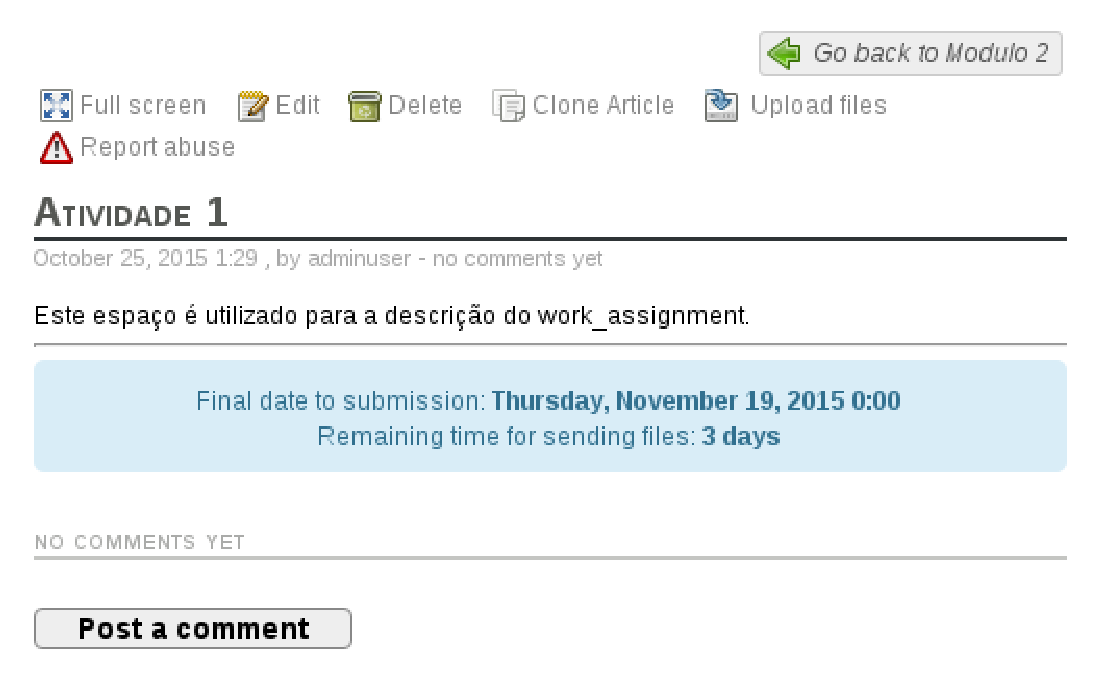
\includegraphics[keepaspectratio=true,scale=0.7]
      {figuras/work-open.eps}
    \caption{Visualização de envio dentro do perído determinado.}
    \label{fig:work-open}
\end{figure}

Nessa sprint foi desenvolvida a história de usuário permite ao administrador definir e modificar um tempo limite para envio dos trabalhos no \textit{plugin work assignment}. No contexto do \textit{plugin} o administrador pode criar um novo tipo de conteúdo ``Trabalho a ser entregue'', nesta opção deve informar qual é o tempo limite para que o envio de arquivos. Em seguida, buscando a melhor forma de visualização para os usuários foram criados alertas que informam o tempo definido para aquela atividade e o tempo ainda restante para o término do envio, como pode ser vizualizado na figura \ref{fig:work-open}.

\begin{figure}[h]
    \centering
    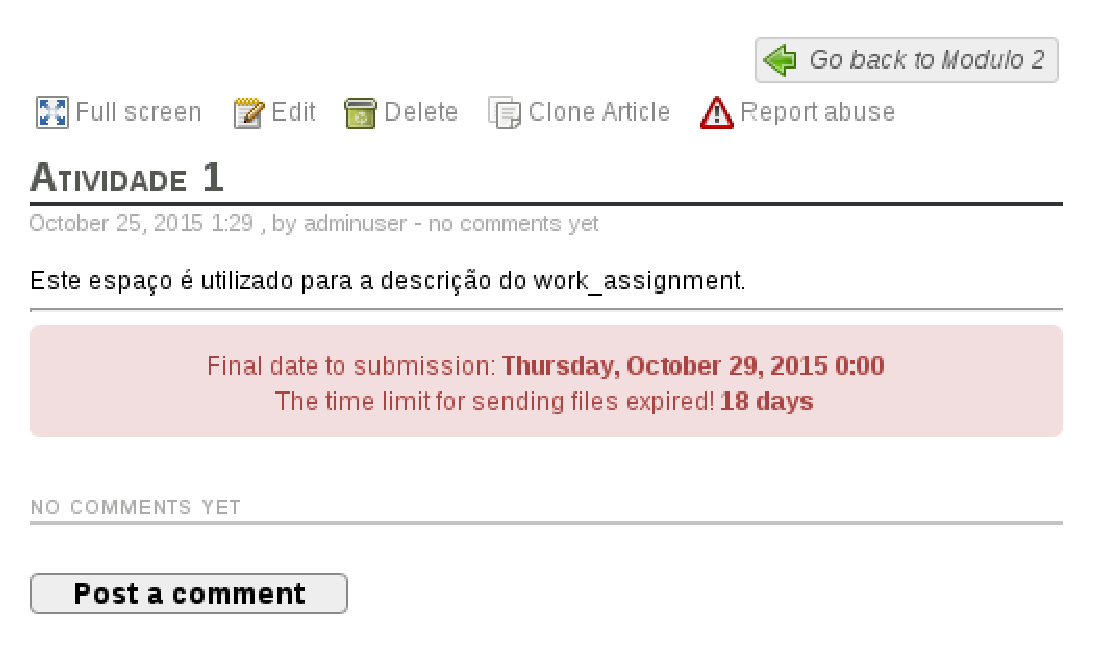
\includegraphics[keepaspectratio=true,scale=0.7]
      {figuras/work-expired.eps}
    \caption{Visualização após a data de envio ter expirado.}
    \label{fig:work-expired}
\end{figure}

Seguindo a mesma linha raciocínio, o usuário será informado se o período de envio já expirou e quanto tempo já se passou após a data limite. Na figura \ref{fig:work-expired} é possível visualizar tal funcionalidade implementada.

Na segunda sprint, foi densenvolvido a alguns critérios de aceitação da primeira história que até então não haviam sido resolvidos. Implementou-se o critério que possibilita ao professor permitir aos alunos que enviem suas atividades após o prazo definido. Além de implementar a história que trata o modo de visualização do tempo ainda restante para envio das atividades.

\begin{figure}[h]
    \centering
    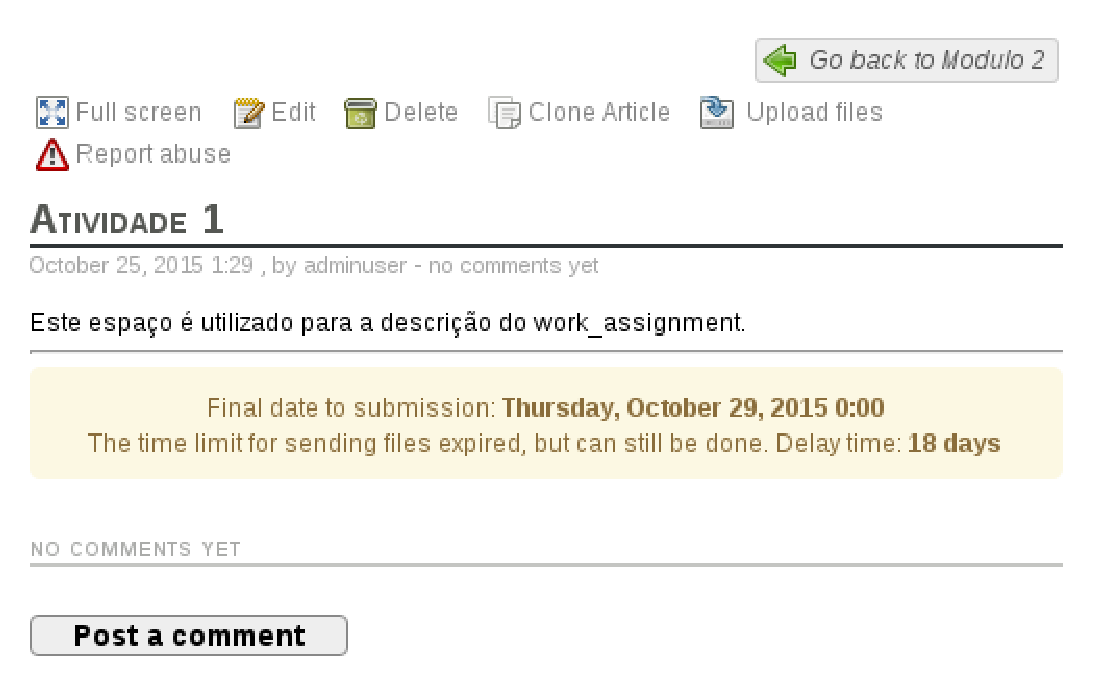
\includegraphics[keepaspectratio=true,scale=0.7]
      {figuras/work-allowed.eps}
    \caption{Visualização de envio após período.}
    \label{fig:work-allowed}
\end{figure}

Em uma discussão com os membros do Lappis foi abordada a melhor maneira para que o usuário visualize a atividade e saiba de imediato em qual situação ela se encontra. Para isso foi utilizado um esquema de cores que fica como plano de fundo do tempo ainda restante. Assim sendo, foram utilizadas três cores: o verde para representar que a atividade está em aberto (Figura \ref{fig:work-open}), o vermelho para indicar que está fechada (Figura \ref{fig:work-expired}) e o laranja para informar que apesar do tempo ter expirado o envio ainda é permitido (Figura \ref{fig:work-allowed}).

É importante ressaltar que na implementação dessa história tem-se um exemplo prático de utilização dos \textit{hotspots} da arquitetura do Noosfero. No código \ref{cod:hotspot}, faz-se uso do \textit{hotspot} denominado como \textit{content\_remove\_upload} que é utilizado para validar quando a opção de upload de arquivos deve estar habilitada. Este código está contido no plugin e através dos métodos dispatch é invocado pela classe responsável por gerenciar os plugins.

\begin{lstlisting}[language=Ruby, caption={Código de implementação do \textit{hotspot}}, label=cod:hotspot]
  def content_remove_upload(content)
    if content.kind_of?(WorkAssignmentPlugin::WorkAssignment)
      !content.profile.members.include?(context.send(:user)) || (content.expired? && !content.ignore_time)
    end
  end
\end{lstlisting}

\begin{figure}[h]
    \centering
    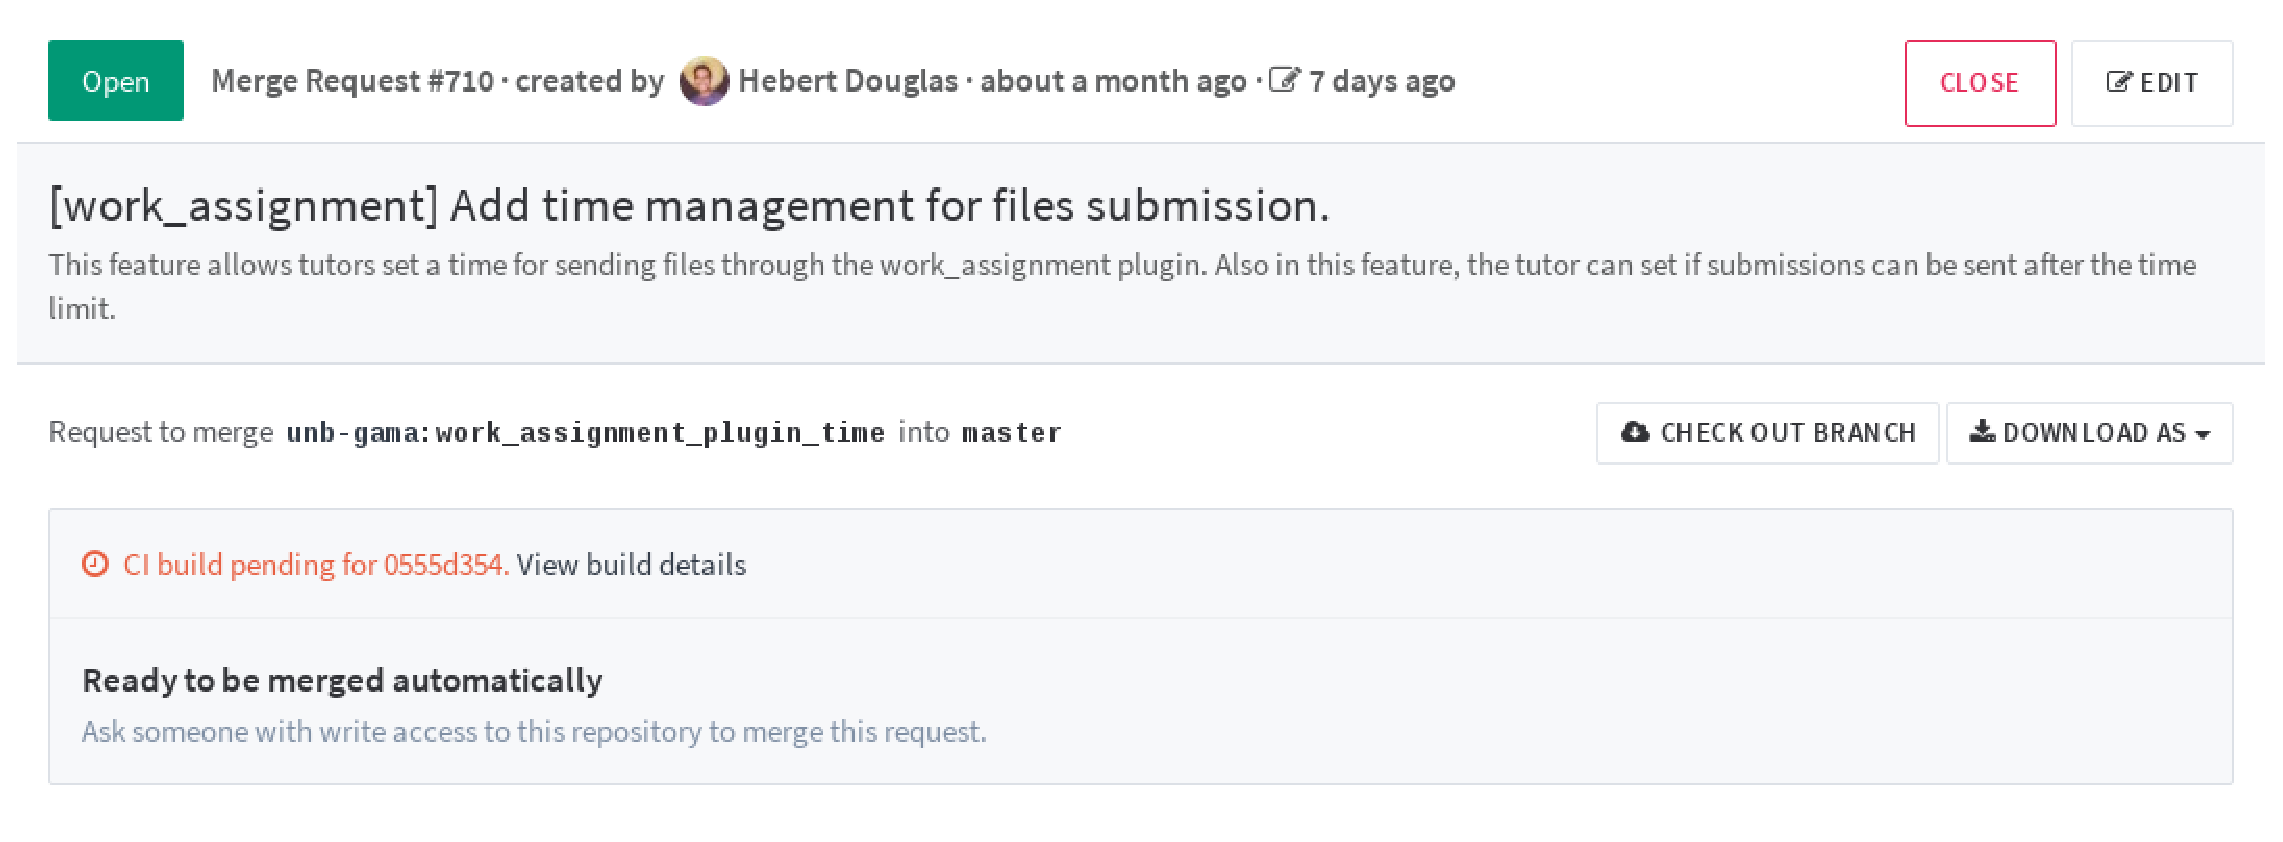
\includegraphics[keepaspectratio=true,scale=0.42]
      {figuras/merge-request710.eps}
    \caption{Merge Request: Gerenciamento de tempo para work\_assignment}
    \label{fig:merge-710}
\end{figure}

A implementação foi revisada por um dos integrantes do Lappis que sugeriu algumas melhorias pontuais, que foram resolvidas durante a revisão. Posteriormente foi realizado o \textit{Merge Request} para a integração do código a \textit{branch \textbf{master}} do Noosfero. Criou-se o Merge Request de número 710\footnote{Disponível em: \url{https://gitlab.com/noosfero/noosfero/merge_requests/710}} (Figura \ref{fig:merge-710}) que ficou em aberto para a revisão dos commiters oficiais da Comunidade. Após alguns dias o mesmo foi revisado pelos desenvolvedores do core do Noosfero, que ainda não alterou o \textit{status} para fechado, mas aprovou a funcionalidade e indicou que se integra ao Noosfero na versão 1\.4.

Nesse processo de desenvolvimento fica evidente a aplicação das práticas adotadas pela comunidade de software livre Noosfero. Foi executado o processo desde a criação de uma \textit{Issue}, passando por todo o processo de desenvolvimento adotando práticas ágeis, até o encerramento desse ciclo com a criação do \textit{Merge request}. Vale lembrar que mesmo após a revisão e integração ao \textit{core} o código ainda se encontra em constante evolução.

Foi iniciada a terceira sprint que engloba a história de ``Atribuir e alterar notas dos arquivos enviados''. No início da implementação verificou-se que esta funcionalidade já havia sido mapeada por integrante do Noosfero na Issue 119 \footnote{Disponível em: \url{https://gitlab.com/noosfero/noosfero/issues/119}}, o que favoreceu o desenvolvimento, pois as idéias poderiam ser discutidas evidenciando que o desenvolvimento na comunidade é feito de maneira colaborativa.

No início de seu desenvolvimento foram discutidas questões técnicas e arquiteturais de como seria a implementação. A principal discussão era como seria a realizada a pontuação, por versões ou por pasta, e como seria estabelecida a nota final do aluno. Foi definido que todas as versões de arquivos enviados poderiam ser pontuados pelos administradores da comunidade e que em uma próxima sprint teriam que ser estabelecidos critérios para julgar qual a nota final do aluno.

\begin{figure}[h]
    \centering
    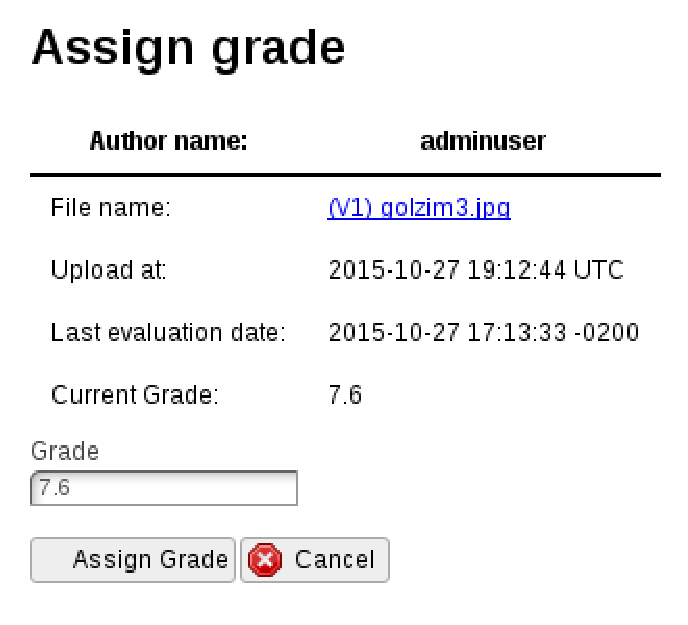
\includegraphics[keepaspectratio=true,scale=0.6]
      {figuras/assign-grade.eps}
    \caption{Tela para atribuição e alteração da notas.}
    \label{fig:assign-grade}
\end{figure}

Para isso foram criados dois atributos (grade\_version, valuation\_date) na classe \textit{UploadFile}, que armazenam a nota da versão enviada e a data da avaliação, assim uma vez que a nota é alterada a data de avaliação é modificada. Na Figura \ref{fig:assign-grade} temos a tela criada para permitir ao administrador atribuir e alterar a nota de cada arquivo enviado.

Na quarta \textit{sprint} foi estabelecido uma forma de implementação que proporciona ao administrador definir qual o critério utilizado para a nota final de cada atividade. Foram determinados três critérios:
\begin{enumerate}
\item Maior nota: é exibida como nota final a maior nota de todas as versões pontuadas.
\item Mais Recente: é exibida como nota final a última versão pontuada.
\item Nota opcional: no momento da avalição de cada versão o administrador define qual é a nota final
\end{enumerate}

Como na arquitetura do \textit{plugin work assignmnet} cada pessoa tem sua pasta com todas as versões de seus arquivos, foi criado na classe \textit{Folder} um método (\textit{final\_grade()}) que verifica qual será nota final de acordo com o critério estabelecido e a associa ao arquivo enviado através do atributo (\textit{grade\_submission\_id}). Esta solução possibilita que uma nota final seja definida mesmo que o professor altere o critério de avaliação.

\begin{figure}[h]
    \centering
    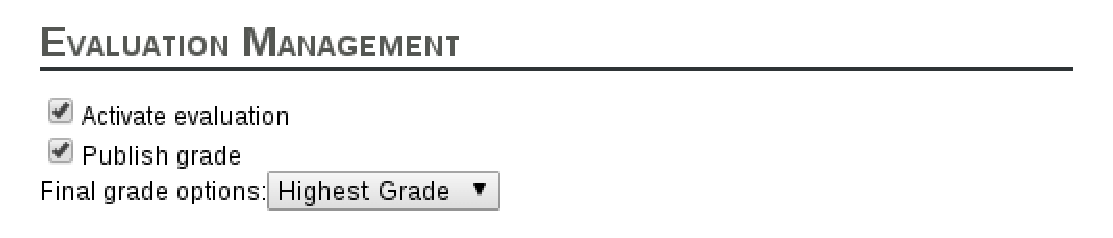
\includegraphics[keepaspectratio=true,scale=0.75]
      {figuras/evaluation-management.eps}
    \caption{Tela para o gerenciamento de avaliações.}
    \label{fig:evaluation-management}
\end{figure}

Ainda nessa \textit{sprint} foi implementada a funcionalidade que permite ao administrador publicar notas aos alunos, como pode ser visualizado na Figura \ref{fig:evaluation-management}. Dessa maneira para cada ``Trabalho a ser enviado'' o administrador pode escolher se deseja ou não publicar as notas para os alunos, que permite ao mesmo realizar todas as avaliações antes de publicá-las.

\begin{figure}[h]
    \centering
    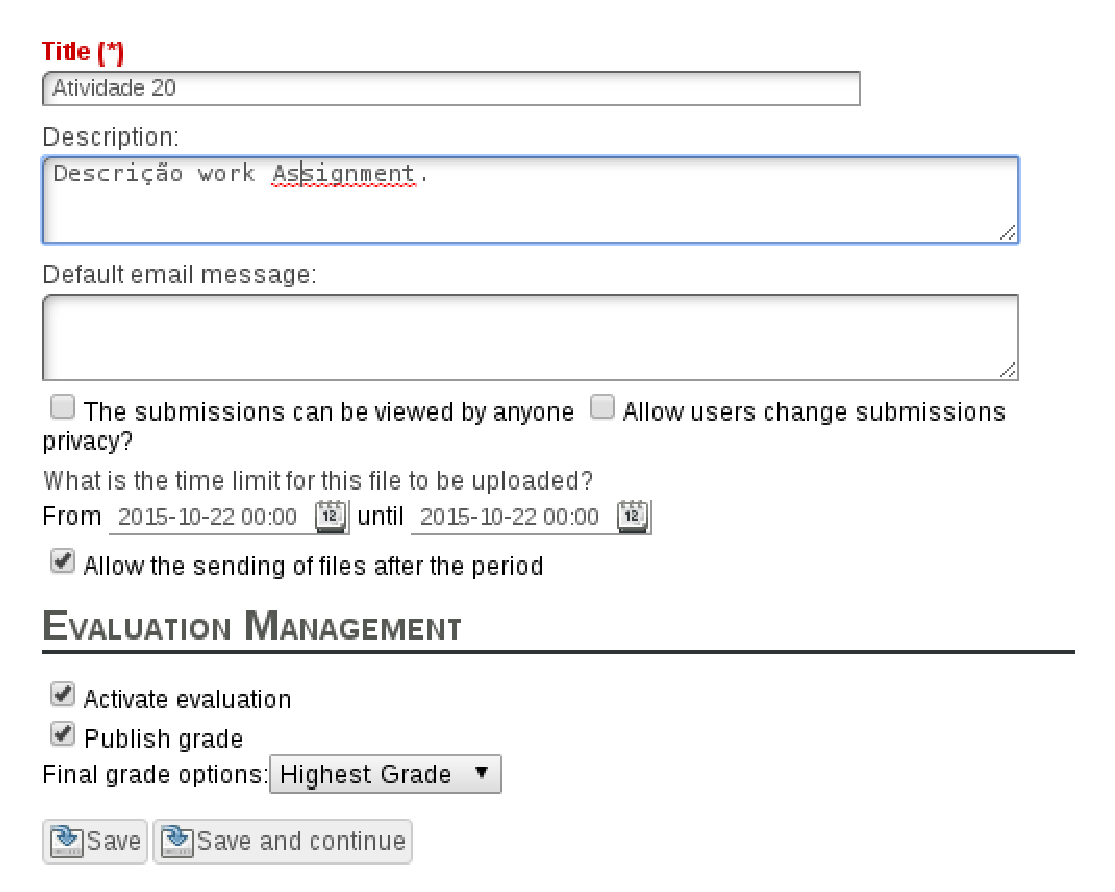
\includegraphics[keepaspectratio=true,scale=0.6]
      {figuras/work-assignment-final.eps}
    \caption{Tela para criação de um \textit{work assignment}.}
    \label{fig:work-assignment-final}
\end{figure}

As funcionalidades desenvolvidas até a quarta \textit{sprint}, englobam requisitos importantes de um AVA, como visto na Seção \ref{ava}. Na Figura \ref{fig:work-assignment-final} é possível verificar como está a página de criação de um novo ``Work Assignment'' após as evoluções realizadas. Dentro desse conteúdo é solicitado ao usuário informações básicas sobre o trabalho, o período que a atividade ficará em aberto e se é possível o envio após a data limite. Na mesma tela temos o gerenciamento das avaliações que permite ativar o modo de avaliação e publicar as notas de acordo com o critério de avaliação.

% Sprint 3

% \item US - Atribuir notas aos alunos;
%     % Atribuir notas
%     % Alterar notas
% Sprint 4
%     % Definir critério da nota final
% \item US - Publicar notas aos alunos;
%     % Disponibilizar notas de uma determinada atividade
%     % Omitir notas de uma determinada atividade

\begin{figure}[h]
    \centering
    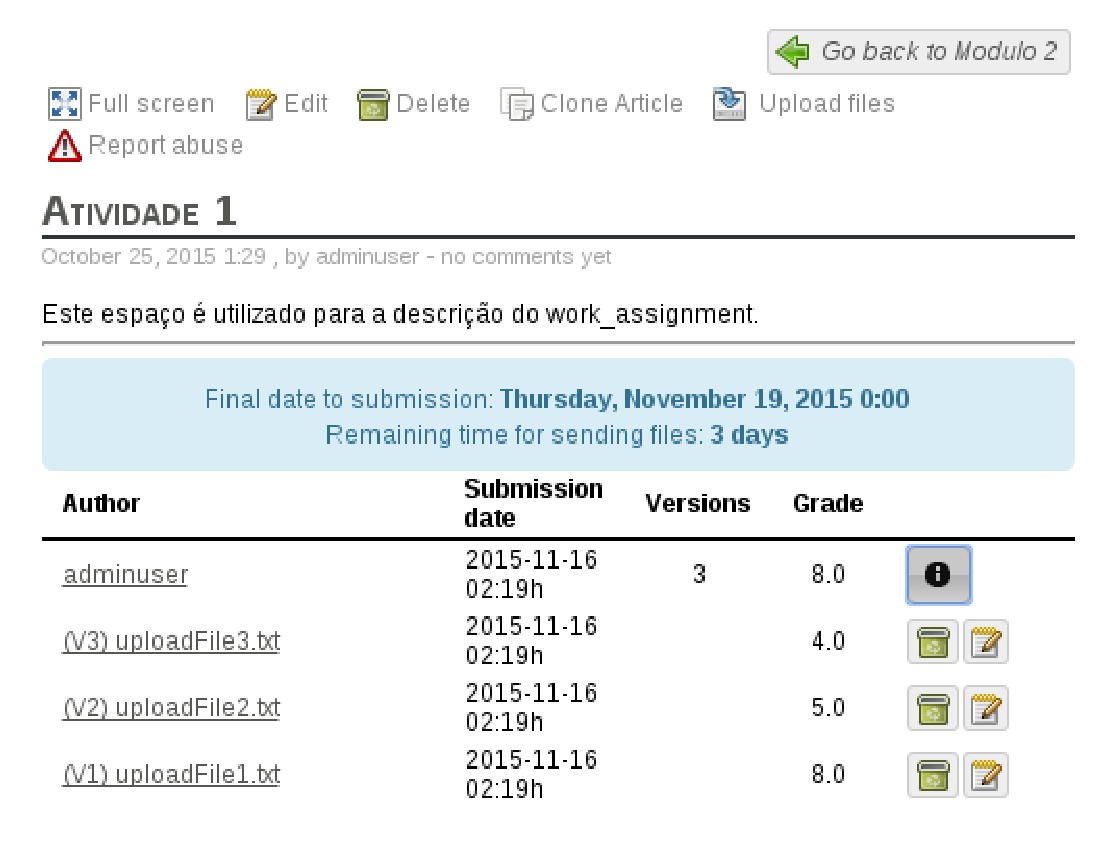
\includegraphics[keepaspectratio=true,scale=0.6]
      {figuras/visualiza-notas.eps}
    \caption{Visualização das notas de trabalhos enviados.}
    \label{fig:visualiza-notas}
\end{figure}

Apesar da implementação das funcionalidades desenvolvidas, até então não era possível a visualização das notas pelo aluno. Assim sendo, na quinta \textit{sprint} foi implementado alguns critérios de aceitação da história de visualização das notas, mostrando apenas as notas na tela de visualização da tarefa enviada. A nível de implementação foi criada uma coluna que é exibida apenas quando a função de envio de notas está habilitada, conforme pode ser verificado na Figura \ref{fig:visualiza-notas}.

Na mesma \textit{sprint} foi implementada a história que permite ao professor definir módulos que agrupem as atividades a serem enviadas, a idéia central é permitir ao administrador modularizar essas atividades. Para isso foi criado uma nova classe \textit{WorkAssignmentPlugin::WorkAssignmentGroup}, que representa um grupo de atividades e tem como funcionalidade básica definir um período para o mesmo.

Com essa nova implementação o administrador da comunidade pode criar módulos ou grupos com data de início e fim, e dentro deles colocar todas as atividades a serem enviadas naquele período. Isto facilita ao professor a organização do curso e permite uma melhor visualização dos alunos.

\begin{figure}[h]
    \centering
    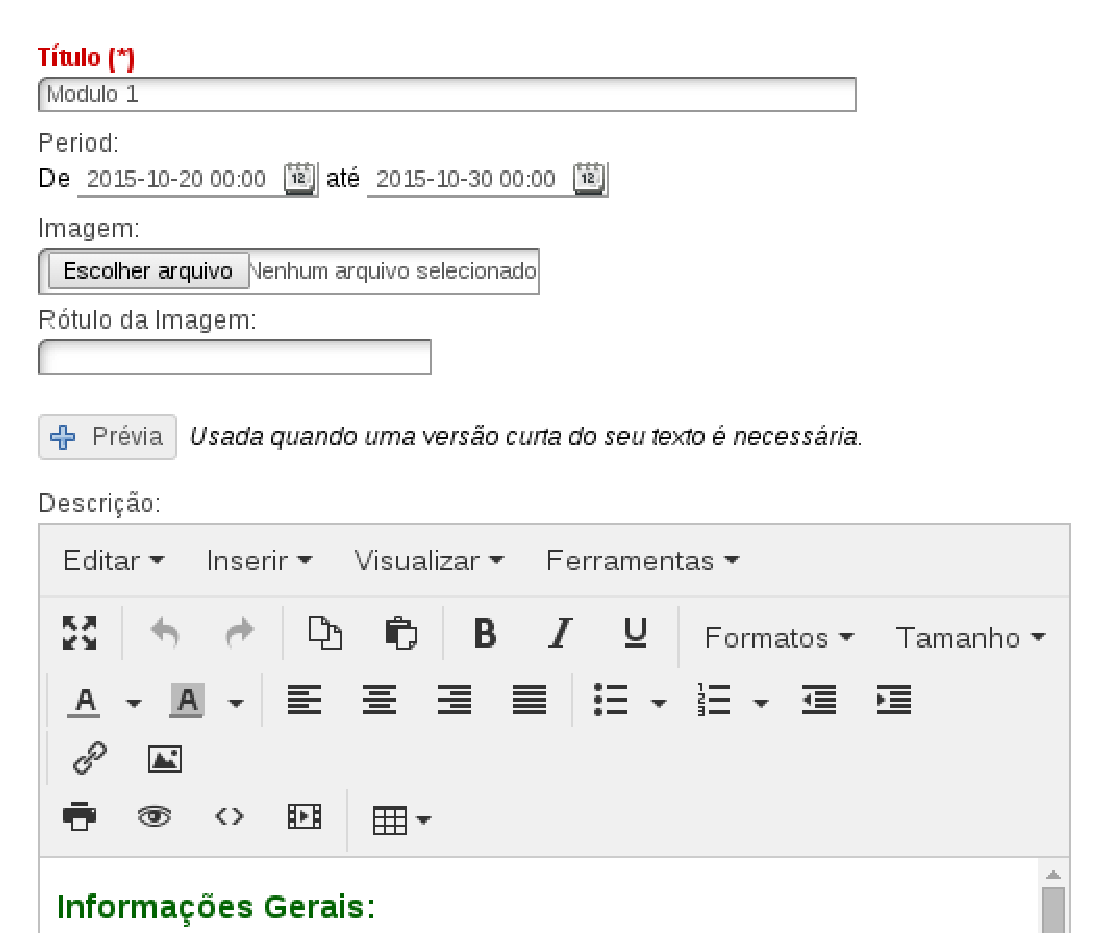
\includegraphics[keepaspectratio=true,scale=0.6]
      {figuras/work-assignment-group.eps}
    \caption{Tela para criação de grupos de trabalhos a serem enviados.}
    \label{fig:work-assignment-group}
\end{figure}

O administrador agora pode entrar no painel de controle da comunidade e adicionar um novo tipo de conteúdo denominado como ``Grupo de Trabalhos a serem enviados''. Dentro desse conteúdo o usuário deve informar o título, período, uma prévia do que será aquele módulo e sua descrição detalhada, conforme pode ser visualizado na Figura \ref{fig:work-assignment-group}

% Sprint 5
% \item US - Aluno visualiza notas;
%     % Visualizar cursos com notas disponíveis
% \item US - Professor gerencia notas;
%     % Definir grupo de atividades


% Sprint 6
% Visualizar notas de todos os alunos de uma determinada atividade
%     % Visualizar notas de todos ao alunos de um grupo de atividades

Na sexta \textit{sprint} foi implementada um forma de visualização das notas de maneira centralizada. A idéia principal é disponibilizar ao usuário todas atividades, agrupadas pelo seus módulos, de todas as comunidades no qual ele é um membro.

\begin{figure}[h]
    \centering
    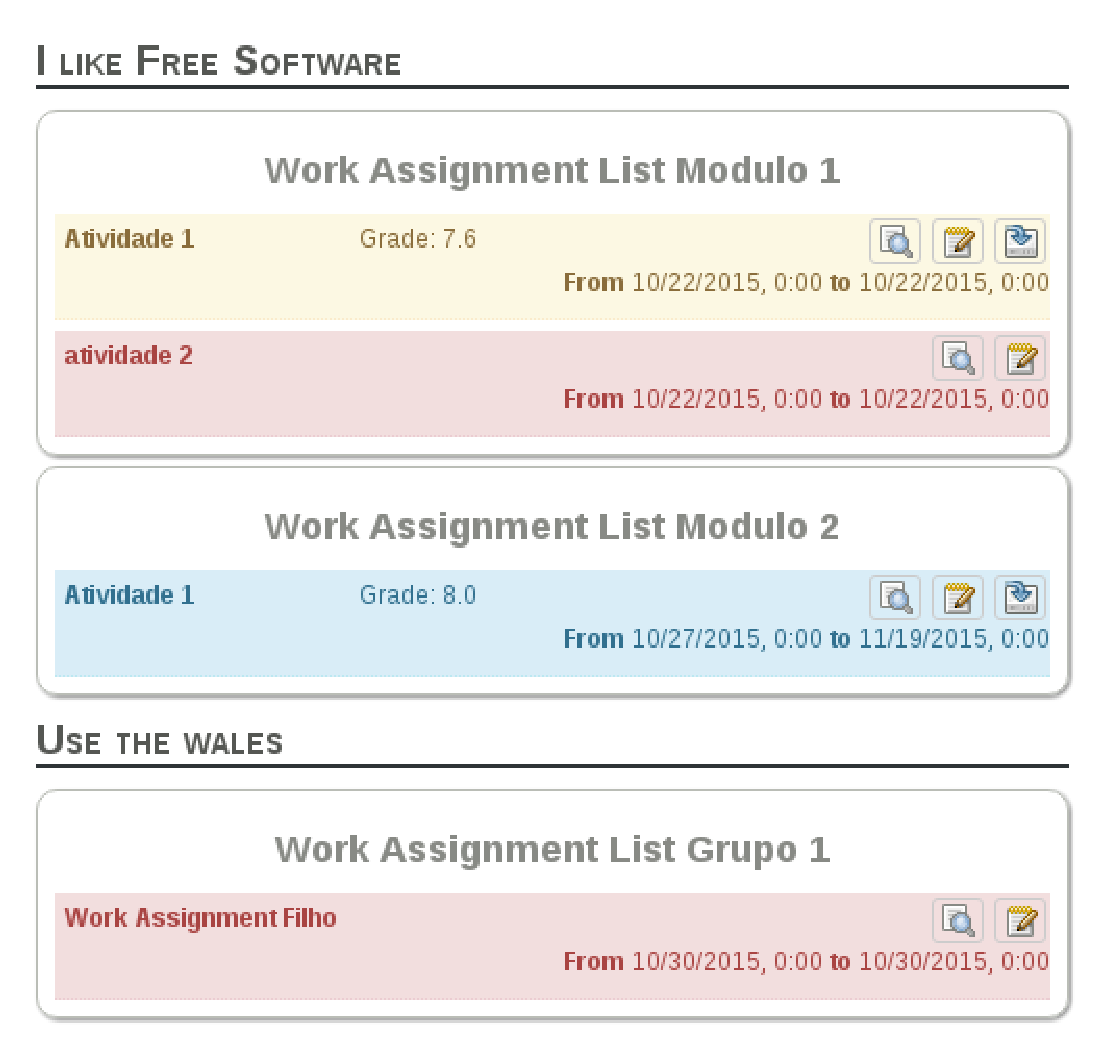
\includegraphics[keepaspectratio=true,scale=0.5]
      {figuras/work-assignment-group-list.eps}
    \caption{Tela para visualização das atividades de forma centralizada.}
    \label{fig:group-list}
\end{figure}

No painel de controle de cada usuário foi criado uma nova funcionalidade chamada de ``Meus Cursos'' que ao ser clicada redireciona o usuário a uma lista de todas as comunidades no qual é membro e utilizam que possuem algum tipo de conteúdo relacionado ao grupo de atividades. Conforme evidenciado na Figura \ref{fig:group-list}, é exibido todas as atidades em seus respectivos grupos.

Durante a implementação dessa história houve uma padronização das \textit{views} utilizadas para visualização das atividades. Dessa maneira, a lista utiliza a mesma lógica de cores proposta anteriormente.

Na sétima \textit{sprint} deu-se prosseguimento com a evolução das telas de visualização, sempre buscando discutir a melhor forma de visualização com os membros da comunidade que trabalham no Lappis. Por conseguinte surgiu a sugestão da implementação de blocos que beneficiaria o usuário quanto ao \textit{feedback} sobre suas notas.

Portanto na mesma \textit{sprint} foi implementada a história para criação de um bloco que exibe ao usuário as cinco notas mais recentes, permitindo ao usuário flexibilidade quanto ao posicionamento e exibição do mesmo.

\begin{figure}[h]
    \centering
    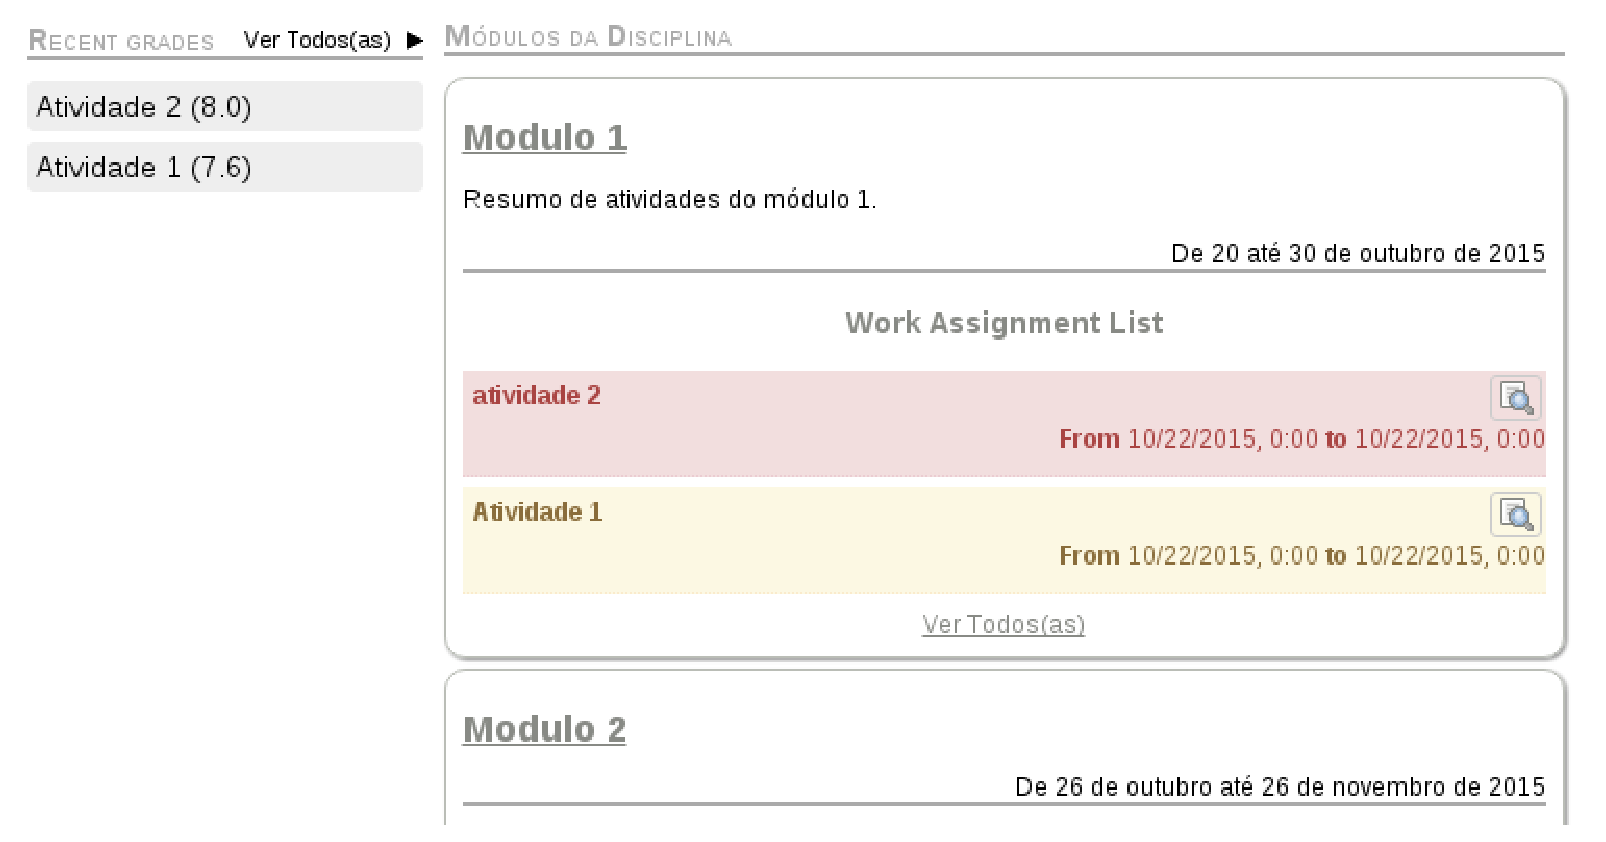
\includegraphics[keepaspectratio=true,scale=0.5]
      {figuras/blocos.eps}
    \caption{Blocos para visualização das atividades.}
    \label{fig:blocos}
\end{figure}

Para oitava \textit{sprint} foi sugerido a criação de um bloco para visualização de todos grupos e suas respectivas atividades. Por padrão são exibidas apenas três atividades por grupo, mas é permitido ao administrador da comunidade escolher quantas deseja. Nessa mesma \textit{sprint} foram realizados os testes para ambos os blocos, afim de verificar e validar a solução. Na figura \ref{fig:blocos} evidencia-se a criação dos blocos em funcionamento.

% Sprint 7
% \item US - Bloco de notas recentes
% -- Adicionar bloco}
% -- Visualizar cinco notas recentes

% Sprint 8
%     \item US - Bloco para visualização dos módulos
%      -- Adicionar bloco}
%      -- Editar numero de atividades listadas no bloco


% \item Ativar autenticação via LDAP UnB;

\section{Arquitetura do Plugin Work Assignment}


Sabendo que o Noosfero está em constante evolução o \textit{plugin work assignment} passará por melhorias durante sua vida útil. Sabendo disso é importante entender sua arquitetura após as implementações realizadas, afim de compreender como quais as classes compõe sua estrutura e como se relacionam.

\begin{figure}[h]
    \centering
    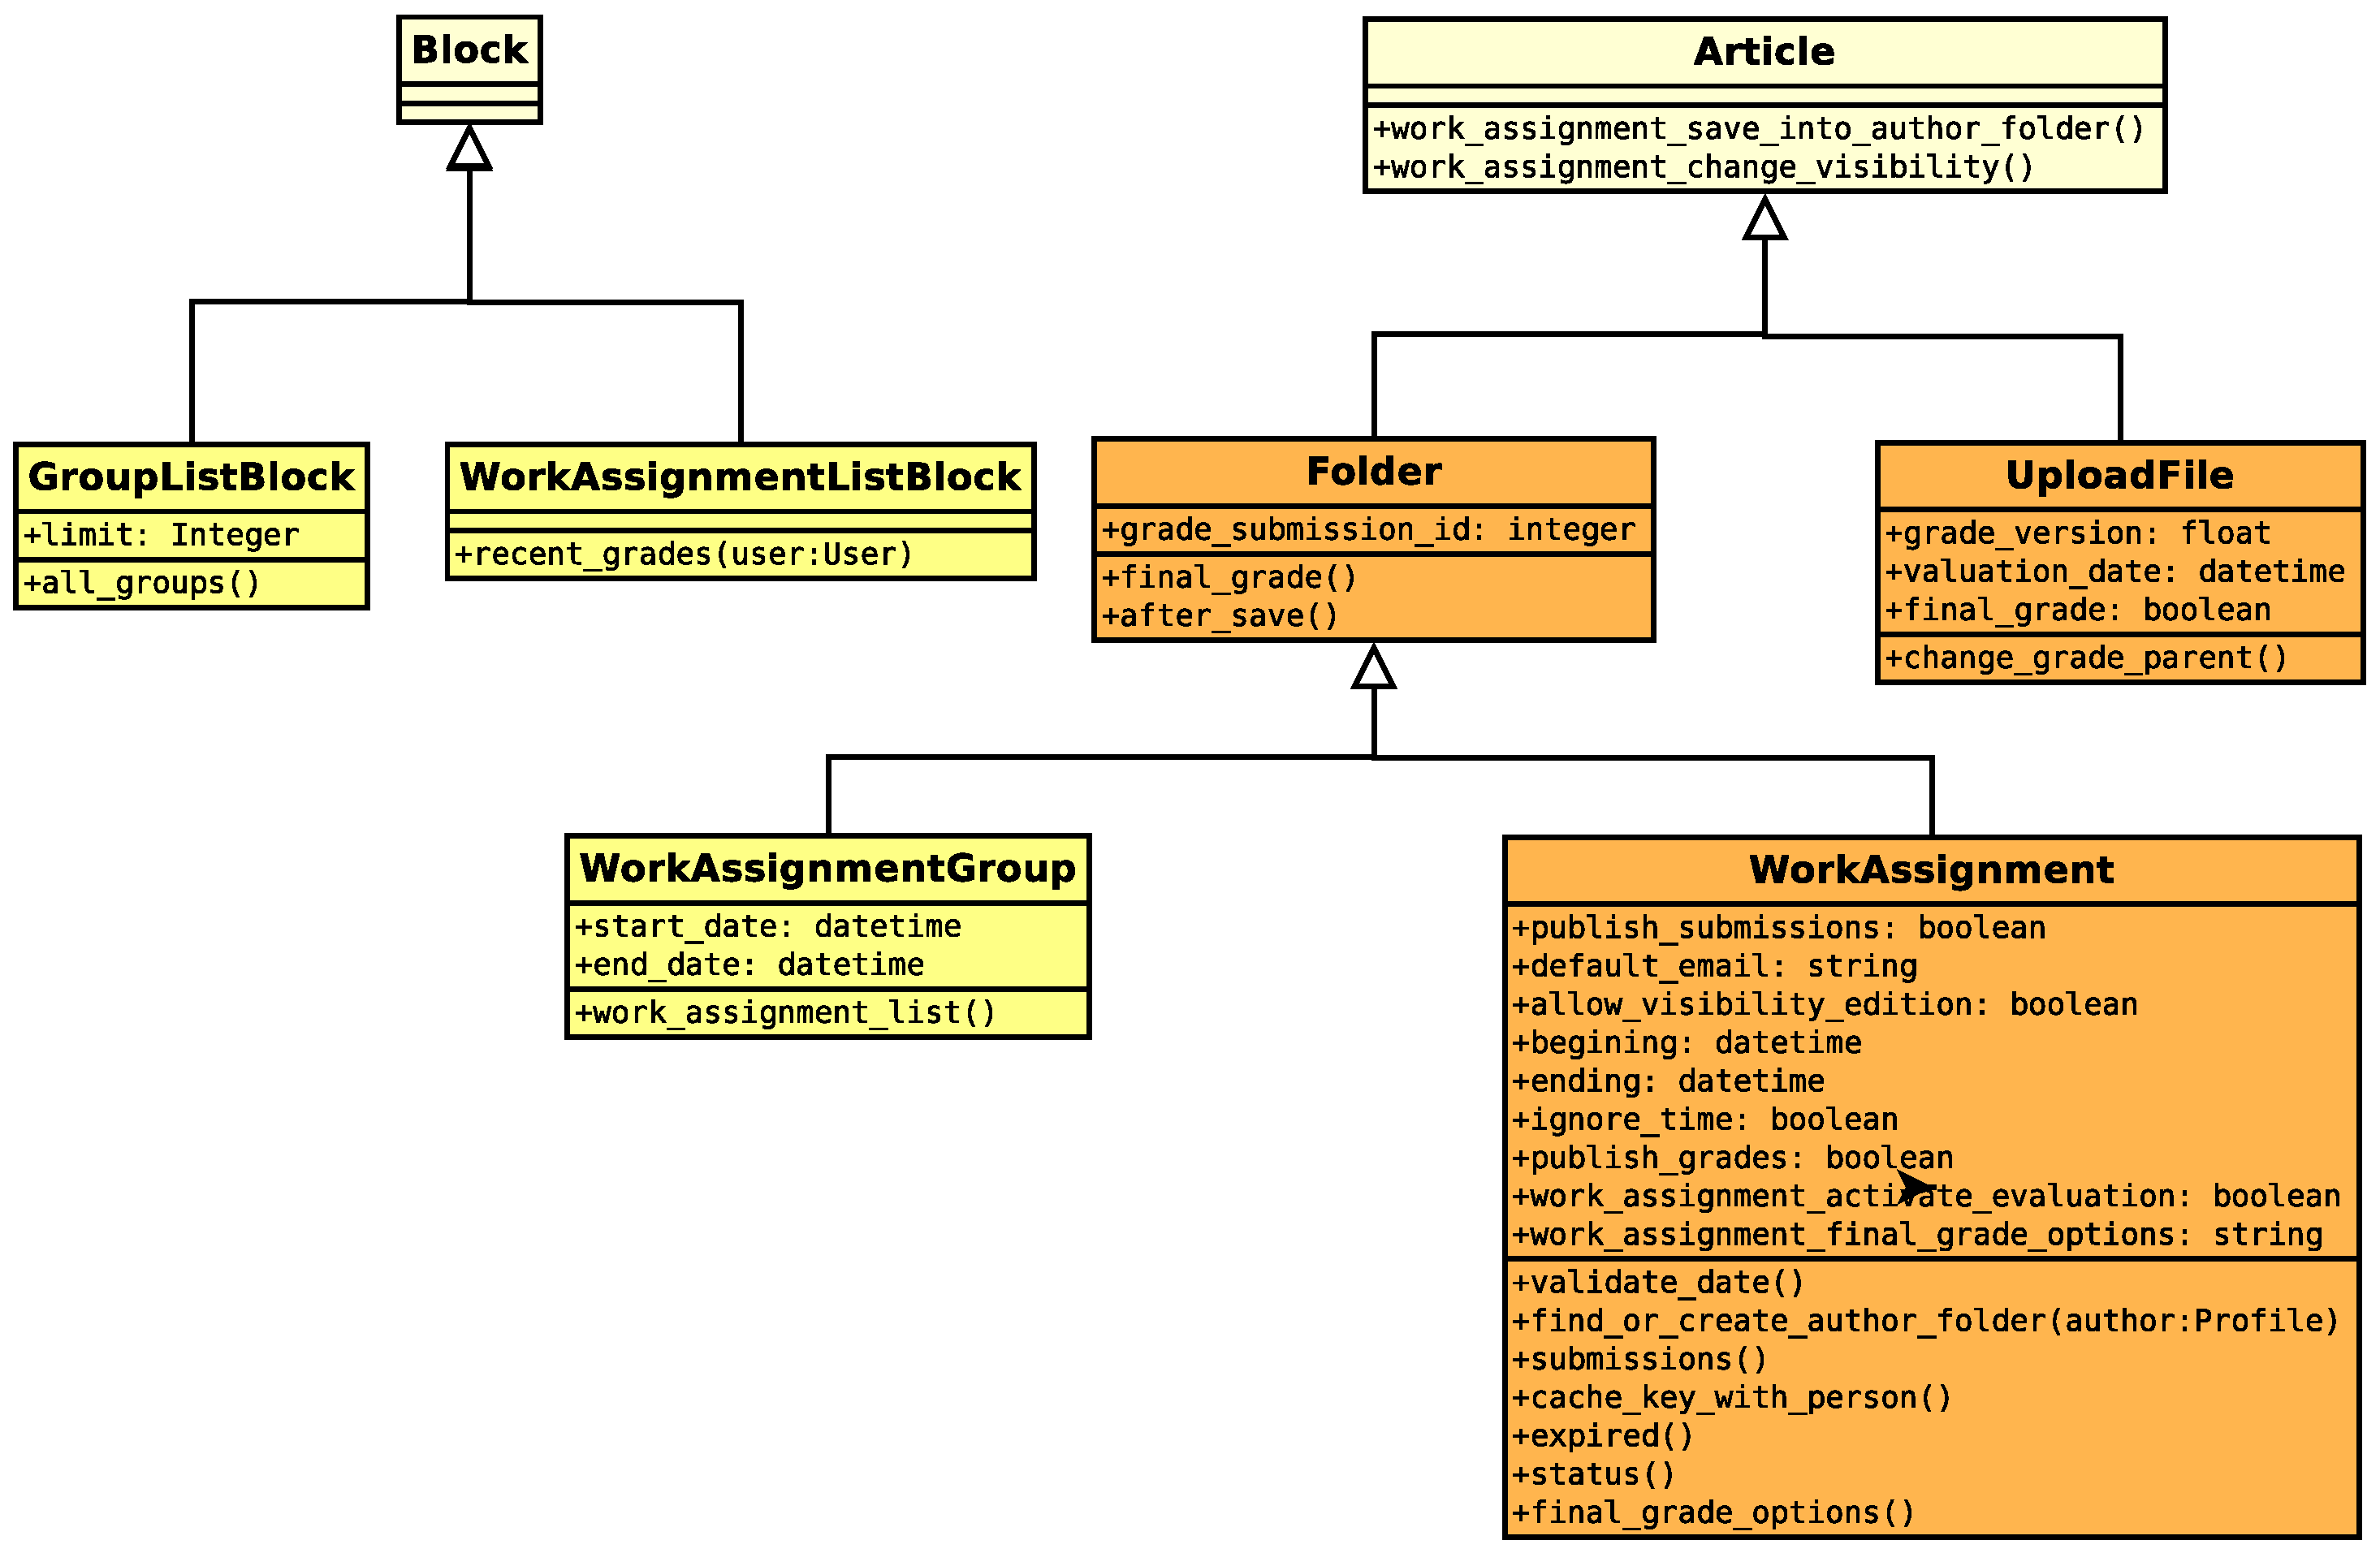
\includegraphics[keepaspectratio=true,scale=0.3]
      {figuras/diagramaUMLCompletoColor.eps}
    \caption{Diagrama de classes do \textit{Plugin Work Assignment}}
    \label{fig:arquitetura-work}
\end{figure}

A Figura \ref{fig:arquitetura-work} evidencia as principais classes utilizadas pelo \textit{plugin}, no qual as que estão em amarelo (tom escuro) foram criadas, as em laranja foram apenas modificadas e por fim as em amarelo (tom claro) não sofreram modificações durante este processo de evolução.

Foi criado mais uma especialização da classe \textit{Folder} denominada como \textit{WorkAssignmentGroup}, que possibilita ao administrador criar pastas que representam grupos de atividades quem tem data de início e fim.

Para entender o funcionamento quando um usuário cria um Grupo de Atividades é possível inserir qualquer tipo de \textit{Article} dentro dessa pasta, dessa maneira é possível criar um Trabalho a ser enviado (\textit{WorkAssignment}. A partir disso os membros da comunidade podem enviar seus arquivos como resposta a atividade, e quando esse envio é realizado o \textit{plugin} cria uma pasta (\textit{Folder}) para cada usuário e a associa ao arquivo enviado (\textit{UploadFile}). Na solução foi levado em consideração que todos os arquivos enviados por uma única pessoa poderiam ser pontuados e deixando de forma opcional qual seria o critério para a nota final.

As classes \textit{WorkAssignmentListBlock} e \textit{GroupListBlock} são uma especialização de \textit{Block} responsáveis por disponibilizar ao usuário a opção de blocos que exibem as notas recentes e listam todos os grupos de uma comunidade, respectivamente.

Entendendo esse funcionamento verifica-se que a arquitetura tornou o \textit{plugin} flexível ao ponto que todas essas classe principais (\textit{WorkAssignmentGroup, WorkAssignment, UploadFile, Folder}) podem ser criadas independente umas das outras. A dependência está relacionada aos blocos que são dispensáveis caso não exista trabalhos a serem enviados ou grupos de atividades.

% Teams Work_assignment https://gitlab.com/noosfero/noosfero/issues/134